\documentclass[11pt]{article}

\usepackage[a4paper,margin=25mm,headheight=15pt]{geometry}
\usepackage[T1]{fontenc}
\usepackage[utf8]{inputenc}
\usepackage{lmodern}
\usepackage{microtype}
\usepackage{amsmath,amssymb,amsthm,mathtools,bm,mathrsfs}
\allowdisplaybreaks
\usepackage{booktabs,longtable,array,tabularx,multirow}
\usepackage{enumitem}
\usepackage{graphicx}
\usepackage{float}
\usepackage{xcolor}
\usepackage{xurl}
\usepackage{listings}
\usepackage{fancyhdr}
\usepackage{caption}
\usepackage{subcaption}
\usepackage{hyperref}
\usepackage[nameinlink,capitalise,noabbrev]{cleveref}

\definecolor{navy}{HTML}{12355B}
\definecolor{teal}{HTML}{187A80}
\definecolor{gold}{HTML}{B7791F}
\definecolor{darkgreen}{HTML}{216E39}
\definecolor{darkred}{HTML}{9B2C2C}
\definecolor{softblue}{HTML}{EDF4FA}
\definecolor{softgreen}{HTML}{EDF7EF}
\definecolor{softgold}{HTML}{FFF8E8}
\definecolor{softred}{HTML}{FFF0F0}
\definecolor{codegray}{HTML}{F5F6F8}
\definecolor{rulegray}{HTML}{AAB2BD}

\hypersetup{
  pdftitle={Dyadic Self-Sampling, Alias Superconvergence, and Rvachev-Appell Deconvolution},
  pdfauthor={OpenAI research synthesis for the ProveIt Fabius-function corpus},
  pdfsubject={New frontier results for the Fabius function, Rvachev up-function, Thue-Morse sequence, q-binomial arithmetic, Bernoulli and Bell polynomials, and Richardson extrapolation},
  pdfkeywords={Fabius function, inverse Fabius function, Rvachev up-function, Thue-Morse, q-binomial, sinc product, Lambert W, Bell polynomial, Bernoulli polynomial, Lagrange interpolation, Richardson extrapolation, quadrature},
  colorlinks=true,
  linkcolor=navy,
  citecolor=darkgreen,
  urlcolor=teal
}

\pagestyle{fancy}
\fancyhf{}
\fancyhead[L]{\small Dyadic self-sampling and Rvachev--Appell deconvolution}
\fancyhead[R]{\small\thepage}
\renewcommand{\headrulewidth}{0.35pt}

\numberwithin{equation}{section}
\setcounter{tocdepth}{2}
\setcounter{secnumdepth}{3}
\setlength{\parindent}{1.15em}
\setlength{\parskip}{0.18em}
\setlist[itemize]{leftmargin=1.55em,itemsep=0.25em,topsep=0.4em}
\setlist[enumerate]{leftmargin=1.75em,itemsep=0.25em,topsep=0.4em}
\setlength{\emergencystretch}{3em}

\newtheorem{theorem}{Theorem}[section]
\newtheorem{proposition}[theorem]{Proposition}
\newtheorem{lemma}[theorem]{Lemma}
\newtheorem{corollary}[theorem]{Corollary}
\newtheorem{claim}[theorem]{Claim}
\newtheorem{conjecture}[theorem]{Conjecture}
\newtheorem{problem}[theorem]{Problem}
\theoremstyle{definition}
\newtheorem{definition}[theorem]{Definition}
\newtheorem{example}[theorem]{Example}
\newtheorem{experiment}[theorem]{Computer-assisted experiment}
\theoremstyle{remark}
\newtheorem{remark}[theorem]{Remark}
\newtheorem{warning}[theorem]{Warning}

\newenvironment{resultbox}[1][]
{\begin{center}\begin{minipage}{0.94\textwidth}%
\color{navy}\hrule height 0.8pt\vspace{0.45em}%
\color{black}\textbf{#1}\par\smallskip}
{\vspace{0.35em}\color{navy}\hrule height 0.5pt\end{minipage}\end{center}}

\newenvironment{statusbox}[1][]
{\begin{center}\begin{minipage}{0.94\textwidth}%
\color{darkgreen}\hrule height 0.8pt\vspace{0.45em}%
\color{black}\textbf{#1}\par\smallskip}
{\vspace{0.35em}\color{darkgreen}\hrule height 0.5pt\end{minipage}\end{center}}

\newenvironment{conjecturebox}[1][]
{\begin{center}\begin{minipage}{0.94\textwidth}%
\color{gold!80!black}\hrule height 0.8pt\vspace{0.45em}%
\color{black}\textbf{#1}\par\smallskip}
{\vspace{0.35em}\color{gold!80!black}\hrule height 0.5pt\end{minipage}\end{center}}

\lstdefinestyle{frontiercode}{
  language=Python,
  basicstyle=\ttfamily\footnotesize,
  backgroundcolor=\color{codegray},
  frame=single,
  rulecolor=\color{rulegray},
  breaklines=true,
  columns=fullflexible,
  showstringspaces=false,
  keywordstyle=\color{navy}\bfseries,
  commentstyle=\color{teal},
  stringstyle=\color{gold!85!black},
  xleftmargin=0.5em,xrightmargin=0.5em,
  aboveskip=0.8em,belowskip=0.8em
}

\DeclareMathOperator{\supp}{supp}
\DeclareMathOperator{\sgn}{sgn}
\DeclareMathOperator{\Var}{Var}
\DeclareMathOperator{\Res}{Res}
\DeclareMathOperator{\ord}{ord}
\DeclareMathOperator{\lcm}{lcm}
\DeclareMathOperator{\DFT}{DFT}
\newcommand{\R}{\mathbb R}
\newcommand{\Q}{\mathbb Q}
\newcommand{\Z}{\mathbb Z}
\newcommand{\N}{\mathbb N}
\newcommand{\C}{\mathbb C}
\newcommand{\E}{\mathbb E}
\newcommand{\eps}{\varepsilon}
\newcommand{\Up}{\operatorname{up}}
\newcommand{\sincpi}{\operatorname{sinc}_{\pi}}
\newcommand{\dd}{\,\mathrm d}
\newcommand{\e}{\mathrm e}
\newcommand{\iu}{\mathrm i}
\newcommand{\bigO}{\mathrm O}
\newcommand{\smallo}{\mathrm o}
\newcommand{\floor}[1]{\left\lfloor#1\right\rfloor}
\newcommand{\ceil}[1]{\left\lceil#1\right\rceil}
\newcommand{\abs}[1]{\left|#1\right|}
\newcommand{\norm}[1]{\left\lVert#1\right\rVert}
\newcommand{\qbinom}[3]{\genfrac{[}{]}{0pt}{}{#1}{#2}_{#3}}
\newcommand{\Bper}{\widetilde B}
\newcommand{\Acal}{\mathscr A}
\newcommand{\Kcal}{\mathcal K}
\newcommand{\Qcal}{\mathcal Q}
\newcommand{\Mcal}{\mathcal M}
\newcommand{\Pcal}{\mathcal P}
\newcommand{\repo}{\textsc{ProveIt}}
\newcommand{\statusproved}{\textcolor{darkgreen}{\textbf{proved here}}}
\newcommand{\statuscomputer}{\textcolor{gold!75!black}{\textbf{computer-assisted, exact arithmetic}}}
\newcommand{\statusconjectural}{\textcolor{darkred}{\textbf{conjectural}}}

\begin{document}
\hypersetup{pageanchor=false}
\pagenumbering{gobble}

\begin{titlepage}
\centering
\vspace*{1.0cm}
{\color{navy}\rule{0.84\textwidth}{1.2pt}}\\[0.95cm]
{\Huge\bfseries\color{navy} Dyadic Self-Sampling,\\[0.18em]
Alias Superconvergence, and\\[0.18em]
Rvachev--Appell Deconvolution\par}
\vspace{0.65cm}
{\Large\color{teal}Frontier results linking the Fabius and inverse Fabius functions,\\
Thue--Morse spectral signs, $q$-binomial arithmetic, Bernoulli kernels,\\
Bell-polynomial zero jets, and positive Richardson filters\par}
\vspace{0.9cm}
{\color{navy}\rule{0.84\textwidth}{0.6pt}}\\[1.15cm]
{\large OpenAI research synthesis\par}
\vspace{0.25cm}
{\large 27 August 2026\par}
\vfill
\begin{minipage}{0.90\textwidth}
\small
\textbf{Research status.}
The self-sampling theorem, its alias expansion, the exact first-defect formula, the Bernoulli convolution identity, the phase-superconvergence classification for all sufficiently fine levels, the positive coset/Richardson construction, the inverse-moment Rvachev--Appell calculus, and the finite $q$-binomial corollaries are proved in this report.  The first failure of real-rootedness for the new Appell family is certified by an exact Sturm count and is explicitly marked computer-assisted.  All proposed endpoint, denominator, and higher-defect statements are labeled as conjectures or research problems.  ``New'' always means new relative to the audited repository snapshot; no claim of worldwide priority is made.
\end{minipage}
\vfill
\end{titlepage}

\clearpage
\hypersetup{pageanchor=true}
\pagenumbering{roman}

\begin{abstract}
Let $u=\Up$ be Rvachev's even $C^\infty$ probability density on $[-1,1]$ and let
\[
 \Phi(\xi)=\widehat u(\xi)
 =\prod_{j=0}^{\infty}\sincpi\!\left(\frac{\xi}{2^j}\right),
 \qquad \sincpi z=\frac{\sin(\pi z)}{\pi z}.
\]
The zero of $\Phi$ at a nonzero integer $m$ has multiplicity $1+\nu_2(m)$.  We show that this elementary zero geometry contains a previously unstated positive quadrature theory.  For every level $N\ge0$, every phase $\theta\in\R$, and every polynomial $p$ of degree at most $N$,
\[
 \int_{-1}^{1}p(x)u(x)\dd x
 =2^{-N}\sum_{k\in\Z}
 p\!\left(\frac{k+\theta}{2^N}\right)
 u\!\left(\frac{k+\theta}{2^N}\right).
\]
The sum is finite and its weights are positive.  At dyadic phases all nodes and weights are rational, so the formula converts exact Fabius values into positive rational moment rules.  Poisson summation gives an entire master alias identity.  Its first nonzero Taylor coefficient is an exact half-integer Fourier series whose signs are the Thue--Morse sequence.  The same defect is a periodic convolution of a Bernoulli polynomial with the rescaled up-function.  First-harmonic dominance identifies the only superconvergent phases from level $N\ge2$ onward: centered or half-shifted phases when $N$ is even, and quarter phases when $N$ is odd.  These rules are positive and exact through degree $N+1$.

Averaging all $2^s$ dyadic phase classes produces the finer level $N+s$ rule.  In alias space this is the unique full residue-class filter gaining $s$ degrees; in physical space it is a positive analogue of Richardson extrapolation.  We then introduce the inverse-moment Rvachev--Appell polynomials
\[
 \frac{\e^{xz}}{M(z)}=\sum_{n\ge0}\Acal_n(x)\frac{z^n}{n!},
 \qquad
 M(z)=\int\e^{zx}u(x)\dd x.
\]
Their coefficients are complete Bell polynomials in explicit Bernoulli cumulants.  They deconvolve the up-law and turn every self-sampling rule into an exact finite translation formula for ordinary monomials.  Exact Sturm arithmetic shows that $\Acal_8$ has four real and four nonreal zeros, so a natural real-rootedness guess fails at degree eight.

Finally, substituting the repository's Gaussian-$q$-binomial--Thue--Morse formula for every dyadic weight yields finite identities equating $q$-binomial digital sums to Bell-polynomial moments.  Transport through the inverse Fabius function gives a rational quadrature family for the nonlinear quantile class $p(2F^{-1}(t)-1)$.  The report closes with conjectures on exact superconvergent precision, the next alias layer, denominator valuations, Appell zero geometry, Lambert-$W$ endpoint sum rules, multidimensional cubature, and Lean formalization.
\end{abstract}

\tableofcontents
\clearpage
\pagenumbering{arabic}

\section{Scope, corpus audit, and novelty boundary}
\label{sec:scope}

\subsection{What was read}

The documentation tree is not a single article.  It contains a living primary exposition, a mathematical glossary, a Lean walkthrough, a non-elementarity paper, a consolidated non-formalized frontier volume, a large Thue--Morse formula atlas, twelve mutually auditing Fourier-decay dossiers, seven imported TeX source papers, and a frozen archive of earlier variants and topic studies.  The audit followed the repository's own provenance convention: living manuscripts were treated as authoritative current statements; active competing drafts were retained separately because their hypotheses and correction histories differ; byte-identical or superseded archive copies were used as historical negative controls rather than counted as independent evidence.

The complete ledger contains 57 distinct TeX artifacts: 25 living/current sources and 32 frozen historical sources.  The grouped inventory is reproduced in \cref{app:corpus}.  In addition, the current versions of the primary exposition, frontier volume, formula atlas, Lean walkthrough, and non-elementarity paper were rechecked at the repository snapshot used for this report.

\begin{table}[H]
\centering
\caption{Corpus families used for the nonduplication audit.}
\label{tab:corpus-summary}
\begin{tabularx}{\textwidth}{@{}l r X@{}}
\toprule
Family & TeX files & Material treated as prior art \\
\midrule
Living primary expositions & 4 & Definitions, probability law, exact dyadic values, moments, Fourier product, endpoint asymptotics, terminology, and formalization map.\\
Canonical frontier volume & 1 & Dyadic/asymptotic bridges, repeated integration, inverse analysis, convergence rates, and open-problem register.\\
Living Thue--Morse atlas & 1 & Digital identities, Prouhet cancellation, Mahler equations, Bell/Bernoulli formulas, and rarefaction.\\
Fourier-decay dossier series & 12 & Pointwise and averaged decay, arithmetic rays, zero geometry, exceptional scales, and final audits.\\
Imported source-paper TeX & 7 & Classical up-function, Fabius arithmetic, lacunary products, and automatic-sequence background.\\
Frozen archive & 32 & Earlier notes, parallel expositions, $q$-calculus supplements, inverse drafts, and former frontier reports.\\
\midrule
Total & 57 & Every group and path family is listed in \cref{app:corpus}.\\
\bottomrule
\end{tabularx}
\end{table}

\subsection{Strong negative controls}

The following themes already occur in the corpus and therefore are \emph{not} claimed as new here:
\begin{itemize}
\item exact dyadic evaluation by moments, Gaussian $q$-binomial coefficients, and finite Thue--Morse sums;
\item Bernoulli cumulants and Bell-polynomial reconstruction of moments;
\item zero multiplicity $1+\nu_2(m)$, integer zero jets, half-integer spectral signs, and canonical-product arithmetic;
\item fixed- and rational-ray Fourier-decay analysis, including sharp logarithmic envelopes;
\item lower-Lambert endpoint coordinates, periodic endpoint factors, and inverse-Fabius Lambert--Bell reversion;
\item geometric Lagrange interpolation, ordinary and logarithmic $q$-Richardson acceleration, and positive Gaussian/Lobatto tail rules;
\item the forward ``dyadic Appell'' family generated by $M(z)\e^{xz}$.
\end{itemize}

Those results are used as input or comparison points.  In particular, the Appell family introduced in \cref{sec:appell} is generated by \emph{the reciprocal} $1/M(z)$ and is the umbral inverse of the forward moment family; it is not a renaming of the Appell polynomials already present in the frontier volume.

\subsection{New layer isolated by the audit}

A targeted search of the living and frozen sources found no theorem asserting polynomial exactness of the self-weighted shifted dyadic samples
\[
 2^{-N}u\!\left(\frac{k+\theta}{2^N}\right),
\]
no master shifted-alias generating function for their moment defects, no Bernoulli convolution formula for the first defect, and no classification of positive phase-superconvergent rules.  The search also found no inverse-moment Rvachev--Appell deconvolution family and no exact link from that family to the self-sampling rules.

The responsible novelty statement is therefore:
\begin{quote}
The results below are new relative to the complete audited \repo{} corpus and were not located as an exact combined construction in a targeted literature search.  They should not be read as a claim of global mathematical priority.
\end{quote}

\begin{statusbox}[Principal proved contributions]
The report proves four mutually reinforcing structures:
\begin{enumerate}
\item a positive shifted dyadic quadrature exact through degree $N$ at level $N$;
\item an exact alias/Thue--Morse/Bernoulli description of its first failure, with parity-selected degree-$N+1$ superconvergence;
\item a unique positive coset filter realizing Richardson-type degree gains by phase averaging;
\item an inverse-moment Bell--Bernoulli Appell calculus that deconvolves the up-law and is reproduced exactly by the same finite rules.
\end{enumerate}
\end{statusbox}

\section{Normalization and established structure}
\label{sec:background}

\subsection{The up-law, Fabius function, and Fourier convention}

Let $u=\Up$ be Rvachev's even nonnegative $C^\infty$ function supported on $[-1,1]$, normalized by
\[
 \int_{-1}^{1}u(x)\dd x=1,
 \qquad u(0)=1.
\]
We use
\begin{equation}
 \widehat f(\xi)=\int_{\R}f(x)\e^{-2\pi\iu x\xi}\dd x,
 \qquad
 \Phi(\xi)=\widehat u(\xi)
 =\prod_{j=0}^{\infty}\sincpi\!\left(\frac{\xi}{2^j}\right),
 \label{eq:Phi-product}
\end{equation}
where
\[
 \sincpi z=\begin{cases}\dfrac{\sin(\pi z)}{\pi z},&z\ne0,\\[0.4em]1,&z=0.\end{cases}
\]
The product is entire.  If $m\in\Z\setminus\{0\}$, then
\begin{equation}
 \ord_{\xi=m}\Phi=1+\nu_2(m).
 \label{eq:integer-multiplicity}
\end{equation}
Indeed, the factors indexed by $0\le j\le\nu_2(m)$ vanish simply and all later factors are nonzero.

The standard Fabius distribution function $F:[0,1]\to[0,1]$ is related to $u$ by
\begin{equation}
 u(x)=F(1-\abs{x})\quad (\abs{x}\le1),
 \qquad
 F(t)=u(t-1)\quad(0\le t\le1).
 \label{eq:F-up-relation}
\end{equation}
If $X$ has density $u$, then
\begin{equation}
 \mathbb P(X\le x)=F\!\left(\frac{x+1}{2}\right),
 \qquad -1\le x\le1.
 \label{eq:centered-CDF}
\end{equation}
Thus the centered quantile is
\begin{equation}
 q(t)=2F^{-1}(t)-1.
 \label{eq:centered-quantile}
\end{equation}

\subsection{Moments, moment generating function, and cumulants}

Write
\begin{equation}
 \mu_n=\int_{-1}^{1}x^n u(x)\dd x,
 \qquad c_n=\mu_{2n}.
 \label{eq:moments}
\end{equation}
Odd moments vanish.  The even moments are rational and satisfy
\begin{equation}
 (2n+1)(2^{2n}-1)c_n
 =\sum_{k=0}^{n-1}\binom{2n+1}{2k}c_k,
 \qquad c_0=1.
 \label{eq:moment-recurrence}
\end{equation}
The moment generating function is
\begin{align}
 M(z)
 &=\int_{-1}^{1}\e^{zx}u(x)\dd x
 =\Phi\!\left(\frac{\iu z}{2\pi}\right)\notag\\
 &=\prod_{j=0}^{\infty}
 \frac{\sinh(z/2^{j+1})}{z/2^{j+1}}.
 \label{eq:mgf-product}
\end{align}
Its logarithm has even cumulants
\begin{equation}
 \log M(z)=\sum_{r=1}^{\infty}\kappa_{2r}\frac{z^{2r}}{(2r)!},
 \qquad
 \boxed{\displaystyle
 \kappa_{2r}=\frac{B_{2r}}{2r}\,
 \frac{2^{2r}}{2^{2r}-1}},
 \label{eq:cumulants}
\end{equation}
where $B_n$ are Bernoulli numbers with $B_2=1/6$.  Consequently
\begin{equation}
 \mu_n=Y_n(0,\kappa_2,0,\kappa_4,\ldots,\kappa_n),
 \label{eq:moment-Bell}
\end{equation}
with $Y_n$ the complete exponential Bell polynomial.

\subsection{Exact dyadic arithmetic}

For $0\le a\le2^n$, the corpus gives the finite moment--Thue--Morse formula
\begin{equation}
 F\!\left(\frac a{2^n}\right)
 =\frac{2^{-n(n+1)/2}}{n!}
 \sum_{h=0}^{a-1}\eps_h
 \sum_{k=0}^{\floor{n/2}}
 \binom n{2k}(2a-2h-1)^{n-2k}c_k,
 \label{eq:finite-F-moment}
\end{equation}
where $\eps_h=(-1)^{s_2(h)}$.  In particular every dyadic sample of $F$ and $u$ is rational.  A second exact formula, recalled in \cref{sec:qbinomial}, expresses the same value through Gaussian binomial coefficients at $q=1/2$ and finite signed Thue--Morse power sums.

\section{The shifted dyadic self-sampling theorem}
\label{sec:self-sampling}

\subsection{Definition of the rules}

For $N\ge0$, $h_N=2^{-N}$, and phase $\theta\in\R$, define
\begin{equation}
 Q_{N,\theta}[f]
 :=h_N\sum_{k\in\Z}
 f\bigl(h_N(k+\theta)\bigr)
 u\bigl(h_N(k+\theta)\bigr).
 \label{eq:Q-def}
\end{equation}
Because $u$ is supported on $[-1,1]$, this is a finite sum.  The nodes are equally spaced, but the weights
\begin{equation}
 w_{N,\theta,k}=h_Nu\bigl(h_N(k+\theta)\bigr)
 \label{eq:self-weights}
\end{equation}
are samples of the target density itself.  They are nonnegative and strictly positive at every interior node.

\begin{theorem}[Shifted self-sampling quadrature]
\label{thm:self-sampling}
For every $N\ge0$, every $\theta\in\R$, and every polynomial $p$ with $\deg p\le N$,
\begin{equation}
 \boxed{\displaystyle
 \int_{-1}^{1}p(x)u(x)\dd x
 =2^{-N}\sum_{k\in\Z}
 p\!\left(\frac{k+\theta}{2^N}\right)
 u\!\left(\frac{k+\theta}{2^N}\right).}
 \label{eq:self-sampling-main}
\end{equation}
In particular, $\sum_k w_{N,\theta,k}=1$, so the rule is a positive probability measure matching the first $N$ moments of $u$.
\end{theorem}

\begin{proof}
Let $0\le r\le N$ and set $f_r(x)=x^ru(x)$.  Since $u\in C_c^\infty(\R)$, Poisson summation applies without regularization.  For the shifted lattice,
\begin{equation}
 h_N\sum_{k\in\Z}f_r\bigl(h_N(k+\theta)\bigr)
 =\sum_{\ell\in\Z}\e^{2\pi\iu\ell\theta}
 \widehat f_r(2^N\ell).
 \label{eq:shifted-Poisson}
\end{equation}
Differentiating \eqref{eq:Phi-product},
\begin{equation}
 \widehat f_r(\xi)=\frac{\Phi^{(r)}(\xi)}{(-2\pi\iu)^r}.
 \label{eq:monomial-transform}
\end{equation}
The term $\ell=0$ is $\mu_r$.  If $\ell\ne0$, then \eqref{eq:integer-multiplicity} gives
\[
 \ord_{\xi=2^N\ell}\Phi
 =N+1+\nu_2(\ell)>r,
\]
so $\Phi^{(r)}(2^N\ell)=0$.  Thus every nonzero alias vanishes, proving the identity for monomials and hence for all polynomials of degree at most $N$.
\end{proof}

\begin{remark}[A dyadic Strang--Fix phenomenon]
Classical Strang--Fix conditions turn zeros of a generator's Fourier transform at the dual lattice into polynomial reproduction by shifts.  Here the generator also supplies the quadrature weights.  The result is therefore a self-weighted, positive, shifted Strang--Fix rule rather than a cardinal interpolation formula.  The exact order is read directly from the $2$-adic multiplicities of the sinc product.
\end{remark}

\subsection{Rationality and denominator control}

\begin{corollary}[Positive rational rules]
\label{cor:rational-rules}
If $\theta=a/2^s$ is dyadic, every node and every weight in \eqref{eq:self-sampling-main} is rational.  More explicitly, with
\[
 D=N+s,
 \qquad n_k=2^sk+a,
 \qquad b_k=2^D-\abs{n_k},
\]
one has, whenever $\abs{n_k}<2^D$,
\begin{equation}
 x_k=\frac{n_k}{2^D},
 \qquad
 w_k=2^{-N}F\!\left(\frac{b_k}{2^D}\right)\in\Q_{>0}.
 \label{eq:rational-weights}
\end{equation}
A common denominator for all such weights is obtained by multiplying the repository's level-$D$ dyadic denominator bound by $2^N$.
\end{corollary}

\begin{proof}
Use \eqref{eq:F-up-relation} at the dyadic node $x_k$.  The denominator assertion follows from the established bound
\[
 D!\,2^{\binom{D+1}{2}}(2\floor{D/2}+1)!!
 \prod_{j=1}^{\floor{D/2}}(2^{2j}-1)\,u(n/2^D)\in\N
\]
for $\abs n<2^D$.
\end{proof}

\subsection{Finite moment identities in Fabius values}

For the centered phase $\theta=0$, symmetry yields particularly transparent formulas.  For $r\ge1$ with $2r\le N$,
\begin{equation}
 \boxed{\displaystyle
 c_r=2^{1-N-2rN}
 \sum_{j=1}^{2^N-1}(2^N-j)^{2r}
 F\!\left(\frac j{2^N}\right).}
 \label{eq:centered-moment-F}
\end{equation}
For $r=0$, normalization reads
\begin{equation}
 1=2^{-N}\left(1+2\sum_{j=1}^{2^N-1}F\!\left(\frac j{2^N}\right)\right).
 \label{eq:centered-normalization-F}
\end{equation}
These are positive finite identities: the moment on the left is reconstructed from values of the Fabius function with no alternating coefficients.

\begin{proof}
Apply \cref{thm:self-sampling} to $p(x)=x^{2r}$.  Pair the nodes $\pm k/2^N$, use $u(k/2^N)=F(1-k/2^N)$, and then put $j=2^N-k$.
\end{proof}

\begin{resultbox}[First frontier bridge]
The exact dyadic values in the corpus were previously used primarily as point evaluations, denominator data, or inputs to signed extrapolation.  Equations \eqref{eq:self-sampling-main}--\eqref{eq:centered-moment-F} instead organize them as a hierarchy of positive moment designs.  Fourier zero multiplicities, dyadic rationality, and probability positivity become three faces of one formula.
\end{resultbox}

\section{The master alias function and the $2$-adic error filtration}
\label{sec:alias}

\subsection{An entire generating function for all moment defects}

Define
\begin{equation}
 G_{N,\theta}(z)
 :=Q_{N,\theta}[\e^{zx}]-M(z).
 \label{eq:G-def}
\end{equation}
The coefficient of $z^r/r!$ is exactly the $r$th moment defect
\begin{equation}
 E_{N,r}(\theta)
 :=Q_{N,\theta}[x^r]-\mu_r.
 \label{eq:ENr-def}
\end{equation}

\begin{theorem}[Master shifted-alias identity]
\label{thm:master-alias}
For every $N\ge0$, $\theta\in\R$, and $z\in\C$,
\begin{equation}
 \boxed{\displaystyle
 G_{N,\theta}(z)
 =\sum_{\ell\in\Z\setminus\{0\}}
 \e^{2\pi\iu\ell\theta}
 \Phi\!\left(2^N\ell+\frac{\iu z}{2\pi}\right).}
 \label{eq:master-alias}
\end{equation}
The series is locally normally convergent.  Moreover $G_{N,\theta}$ has a zero of order at least $N+1$ at $z=0$.
\end{theorem}

\begin{proof}
Apply shifted Poisson summation to $f_z(x)=\e^{zx}u(x)$.  Its Fourier transform is
\[
 \widehat f_z(\xi)
 =\Phi\!\left(\xi+\frac{\iu z}{2\pi}\right).
\]
The zero-frequency term is $M(z)$, giving \eqref{eq:master-alias}.  Compact support and smoothness imply the local normal convergence needed to differentiate termwise.  At $z=0$, the summand indexed by $\ell\ne0$ has order
$N+1+\nu_2(\ell)$, so the full sum begins at order $N+1$.
\end{proof}

\begin{corollary}[Valuation filtration of polynomial errors]
\label{cor:valuation-filtration}
For $r>N$,
\begin{equation}
 E_{N,r}(\theta)
 =\frac1{(-2\pi\iu)^r}
 \sum_{a=0}^{r-N-1}
 \sum_{\substack{q\in\Z\setminus\{0\}\\q\ \mathrm{odd}}}
 \e^{2\pi\iu 2^aq\theta}
 \Phi^{(r)}(2^{N+a}q).
 \label{eq:valuation-filtration}
\end{equation}
Thus the excess degree $r-N$ exposes exactly the first $r-N$ layers of the $2$-adic alias tree.
\end{corollary}

\begin{proof}
In the coefficient formula obtained from \eqref{eq:master-alias}, an alias $\ell$ can contribute only if
$N+1+\nu_2(\ell)\le r$.  Write $\ell=2^aq$ with $q$ odd.
\end{proof}

\begin{remark}
The first failure, $r=N+1$, sees only odd aliases.  The next failure, $r=N+2$, sees odd aliases and twice-odd aliases.  Higher defects are therefore not arbitrary: they are a triangular sequence of $2$-adic spectral layers.  This observation will be the basis of the next-defect conjectures in \cref{sec:frontier}.
\end{remark}

\subsection{An exact local factorization at every integer zero}

The integer zero jets can be organized in a form that makes Bell polynomials appear automatically.

\begin{proposition}[Exact local factorization]
\label{prop:local-factorization}
Let $m=2^{d-1}q\ne0$, where $q$ is odd and $d=1+\nu_2(m)$.  Then, for $w$ near $0$,
\begin{equation}
 \boxed{\displaystyle
 \Phi(m+w)
 =-\left(\frac{w}{m+w}\right)^d
 \left(\prod_{j=0}^{d-1}\sincpi\!\left(\frac{w}{2^j}\right)\right)
 \Phi\!\left(\frac q2+\frac{w}{2^d}\right).}
 \label{eq:local-factorization}
\end{equation}
In particular,
\begin{equation}
 \Phi(m+w)=C_mw^d
 \exp\!\left(\sum_{j\ge1}\gamma_j(m)\frac{w^j}{j!}\right),
 \qquad
 C_m=-\frac{\Phi(q/2)}{m^d},
 \label{eq:local-Bell-form}
\end{equation}
where the logarithmic jet $\gamma_j(m)$ is explicit.
\end{proposition}

\begin{proof}
For $0\le j\le d-1$, $m/2^j$ is an integer and
\[
 \sincpi\!\left(\frac{m+w}{2^j}\right)
 =(-1)^{m/2^j}\frac{w}{m+w}
 \sincpi\!\left(\frac{w}{2^j}\right).
\]
The product of the signs is $-1$ because
\[
 \sum_{j=0}^{d-1}\frac m{2^j}=q(2^d-1)
\]
is odd.  The remaining tail is
\[
 \prod_{j=d}^{\infty}\sincpi\!\left(\frac{m+w}{2^j}\right)
 =\Phi\!\left(\frac q2+\frac{w}{2^d}\right).
\]
This proves \eqref{eq:local-factorization}; taking the analytic logarithm after removing $C_mw^d$ gives \eqref{eq:local-Bell-form}.
\end{proof}

The first logarithmic coefficient is especially simple:
\begin{equation}
 \gamma_1(m)=-\frac d m
 +2^{-d}\frac{\Phi'(q/2)}{\Phi(q/2)}.
 \label{eq:gamma1}
\end{equation}
For general $j$,
\begin{equation}
 \gamma_j(m)
 =d(-1)^j\frac{(j-1)!}{m^j}
 +\sum_{h=0}^{d-1}2^{-hj}\ell_j
 +2^{-dj}L_j(q/2),
 \label{eq:gamma-general}
\end{equation}
where
\[
 \ell_j=\left.\frac{\dd^j}{\dd z^j}\log\sincpi z\right|_{z=0},
 \qquad
 L_j(t)=\frac{\dd^j}{\dd t^j}\log\Phi(t).
\]
The universal local coefficients satisfy
\begin{equation}
 \ell_{2r}=-\frac{(2r)!}{r}\zeta(2r),
 \qquad \ell_{2r+1}=0,
 \label{eq:sinc-log-jet}
\end{equation}
so Bernoulli numbers may be substituted through Euler's formula for $\zeta(2r)$.

\begin{corollary}[Bell-polynomial zero jets]
\label{cor:Bell-zero-jets}
With the notation of \cref{prop:local-factorization}, for every $s\ge0$,
\begin{equation}
 \boxed{\displaystyle
 \Phi^{(d+s)}(m)
 =C_m\frac{(d+s)!}{s!}
 Y_s\bigl(\gamma_1(m),\ldots,\gamma_s(m)\bigr).}
 \label{eq:Bell-zero-jets}
\end{equation}
Here $Y_0=1$.  Consequently every layer of \eqref{eq:valuation-filtration} has a finite Bell-polynomial description in half-integer logarithmic derivatives, zeta values, and elementary $2$-adic data.
\end{corollary}

\begin{proof}
Use the defining exponential generating function
\[
 \exp\!\left(\sum_{j\ge1}x_j\frac{w^j}{j!}\right)
 =\sum_{s\ge0}Y_s(x_1,\ldots,x_s)\frac{w^s}{s!}
\]
in \eqref{eq:local-Bell-form} and compare coefficients.
\end{proof}

\begin{resultbox}[Second frontier bridge]
The corpus already contains the integer zero multiplicities and several zero-jet formulas.  The new point here is their use as an \emph{error calculus}: the excess polynomial degree selects a finite set of $2$-adic alias layers, and every derivative on those layers is generated by a complete Bell polynomial.  Bernoulli/zeta data enter locally through $\log\sincpi$, while Thue--Morse data enter globally through the half-integer tail.
\end{resultbox}

\section{The first defect: half-integer spectrum and Thue--Morse signs}
\label{sec:first-defect}

Put
\begin{equation}
 r=N+1,
 \qquad
 E_N(\theta):=E_{N,N+1}(\theta).
 \label{eq:first-defect-def}
\end{equation}
Only odd aliases survive.

\begin{theorem}[Exact first-defect series]
\label{thm:first-defect}
For every $N\ge0$ and $\theta\in\R$,
\begin{equation}
 \boxed{\displaystyle
 E_N(\theta)
 =-\frac{r!}{(-2\pi\iu)^r2^{Nr}}
 \sum_{\substack{\ell\in\Z\setminus\{0\}\\\ell\ \mathrm{odd}}}
 \frac{\Phi(\ell/2)}{\ell^r}
 \e^{2\pi\iu\ell\theta}.}
 \label{eq:first-defect-complex}
\end{equation}
Equivalently, if $r=2s$,
\begin{equation}
 E_N(\theta)
 =\frac{2(-1)^{s+1}r!}{(2\pi)^r2^{Nr}}
 \sum_{\substack{m\ge1\\m\ \mathrm{odd}}}
 \frac{\Phi(m/2)}{m^r}\cos(2\pi m\theta),
 \label{eq:first-defect-even}
\end{equation}
and if $r=2s+1$,
\begin{equation}
 E_N(\theta)
 =\frac{2(-1)^sr!}{(2\pi)^r2^{Nr}}
 \sum_{\substack{m\ge1\\m\ \mathrm{odd}}}
 \frac{\Phi(m/2)}{m^r}\sin(2\pi m\theta).
 \label{eq:first-defect-odd}
\end{equation}
\end{theorem}

\begin{proof}
For $m=2^N\ell$ with $\ell$ odd, \cref{prop:local-factorization} with $d=r$ gives
\begin{equation}
 \Phi^{(r)}(2^N\ell)
 =-\frac{r!\Phi(\ell/2)}{(2^N\ell)^r}.
 \label{eq:first-zero-jet}
\end{equation}
Insert this into \eqref{eq:valuation-filtration}.  Pair positive and negative odd frequencies to obtain the real forms.
\end{proof}

\subsection{The spectral sign is exactly Thue--Morse}

\begin{proposition}[Half-integer sign law]
\label{prop:half-integer-sign}
For $j\ge0$,
\begin{equation}
 \sgn\Phi\!\left(\frac{2j+1}{2}\right)
 =(-1)^{s_2(j)}=\eps_j.
 \label{eq:half-integer-sign}
\end{equation}
Hence the first quadrature defect is a Thue--Morse-signed half-integer spectral Dirichlet series.
\end{proposition}

\begin{proof}
On the positive real axis, $\Phi$ changes sign whenever an integer zero has odd multiplicity.  At the point $(2j+1)/2=j+1/2$, the total number of zero crossings, counted with multiplicity, is
\[
 \sum_{m=1}^{j}\bigl(1+\nu_2(m)\bigr)
 =j+\nu_2(j!)
 =2j-s_2(j),
\]
where the last equality is Legendre's formula $\nu_2(j!)=j-s_2(j)$.  Its parity is therefore $s_2(j)$.  Since $\Phi(1/2)>0$, the claimed sign follows.
\end{proof}

Writing
\begin{equation}
 a_j=\abs{\Phi((2j+1)/2)},
 \label{eq:half-amplitudes}
\end{equation}
we may rewrite the spectral coefficient as $\Phi((2j+1)/2)=\eps_ja_j$.  Thus the signs are purely digital, while the amplitudes record the sinc-product decay.

\subsection{Symmetries}

\begin{corollary}[Phase symmetries]
\label{cor:defect-symmetries}
The first defect is $1$-periodic and satisfies
\begin{equation}
 E_N(-\theta)=(-1)^rE_N(\theta),
 \qquad
 E_N(\theta+1/2)=-E_N(\theta).
 \label{eq:defect-symmetries}
\end{equation}
\end{corollary}

\begin{proof}
The first identity follows from the sine/cosine parity.  The second follows because every frequency in \eqref{eq:first-defect-complex} is odd.
\end{proof}

\section{A Bernoulli convolution formula for the first defect}
\label{sec:bernoulli-kernel}

\subsection{The periodic up-kernel}

Define a $1$-periodic continuous function $\Kcal$ by
\begin{equation}
 \Kcal(t)=2u(2t)-1,
 \qquad -\frac12\le t\le\frac12,
 \label{eq:K-kernel}
\end{equation}
with periodic extension.  Its mean is zero.  For $n\ne0$, its Fourier coefficient is
\begin{equation}
 \widehat{\Kcal}(n)
 =\int_{-1/2}^{1/2}\Kcal(t)\e^{-2\pi\iu nt}\dd t
 =\Phi(n/2).
 \label{eq:K-Fourier}
\end{equation}
In particular the even nonzero coefficients vanish, and the odd coefficients carry the Thue--Morse signs of \cref{prop:half-integer-sign}.

Let $\Bper_r(t)=B_r(\{t\})$ be the periodic Bernoulli polynomial, understood in the standard Fourier/distributional sense when $r=1$.  For $n\ne0$,
\begin{equation}
 \widehat{\Bper_r}(n)=-\frac{r!}{(2\pi\iu n)^r}.
 \label{eq:periodic-Bernoulli-Fourier}
\end{equation}

\begin{theorem}[Bernoulli--Rvachev error kernel]
\label{thm:Bernoulli-convolution}
For $r=N+1$,
\begin{equation}
 \boxed{\displaystyle
 E_N(\theta)=(-1)^r2^{-Nr}
 (\Bper_r*\Kcal)(\theta),}
 \label{eq:Bernoulli-convolution}
\end{equation}
where convolution is on $\R/\Z$.
\end{theorem}

\begin{proof}
Multiply the nonzero Fourier coefficients in \eqref{eq:K-Fourier} and \eqref{eq:periodic-Bernoulli-Fourier}.  The resulting Fourier series is exactly \eqref{eq:first-defect-complex}; the even frequencies vanish automatically.
\end{proof}

\begin{remark}
This formula is not an Euler--Maclaurin expansion with an unspecified remainder.  It is an exact identity.  The universal periodic Bernoulli kernel describes polynomial aliasing, while $\Kcal$ inserts the complete half-integer spectrum of the up-law.  It therefore provides a direct analytical bridge from Bernoulli polynomials to the Rvachev sinc product.
\end{remark}

\subsection{A rigorous first-harmonic bound}

\begin{lemma}[A uniform lower bound at the first half-integer]
\label{lem:phi-half-lower}
\begin{equation}
 \Phi(1/2)>1-\frac{\pi^2}{18}>\frac49.
 \label{eq:phi-half-lower}
\end{equation}
\end{lemma}

\begin{proof}
For $0\le x\le1/2$, $\sincpi x\ge1-\pi^2x^2/6$.  Since all factors are nonnegative,
\[
 \Phi(1/2)
 \ge1-\frac{\pi^2}{6}\sum_{j=0}^{\infty}4^{-(j+1)}
 =1-\frac{\pi^2}{18}.
\]
The final inequality follows from $\pi^2<10$.
\end{proof}

For $r\ge2$,
\begin{equation}
 \sum_{\substack{m\ge3\\m\ \mathrm{odd}}}
 \frac{\abs{\Phi(m/2)}}{m^r}
 \le\sum_{\substack{m\ge3\\m\ \mathrm{odd}}}\frac1{m^r}
 \le\frac{\pi^2}{8}-1<\frac14.
 \label{eq:harmonic-tail-bound}
\end{equation}
Thus the first coefficient is larger than the sum of all remaining absolute coefficients for every $r\ge2$.

\begin{theorem}[Uniform sinusoidal asymptotics]
\label{thm:sinusoidal-asymptotics}
Let $r=N+1$ and define
\begin{equation}
 A_{N,r}=\frac{2r!\Phi(1/2)}{(2\pi)^r2^{Nr}}.
 \label{eq:first-harmonic-amplitude}
\end{equation}
Then, uniformly in $\theta$,
\begin{align}
 E_N(\theta)
 &=(-1)^{r/2+1}A_{N,r}\cos(2\pi\theta)
 +\bigO\!\left(A_{N,r}3^{-r}\right),&&r\ \text{even},
 \label{eq:cos-asymptotic}\\
 E_N(\theta)
 &=(-1)^{(r-1)/2}A_{N,r}\sin(2\pi\theta)
 +\bigO\!\left(A_{N,r}3^{-r}\right),&&r\ \text{odd}.
 \label{eq:sin-asymptotic}
\end{align}
The implied constant is absolute.
\end{theorem}

\begin{proof}
Separate the frequency $m=1$ in \eqref{eq:first-defect-even} or \eqref{eq:first-defect-odd}.  Since $\abs{\Phi(m/2)}\le1$ and
$\sum_{m\ge3,\,m\text{ odd}}m^{-r}=\bigO(3^{-r})$, the remaining series has the stated uniform bound.
\end{proof}

The exact numerical ratios are far smaller than the elementary majorant:
\begin{table}[H]
\centering
\caption{Absolute spectral tail divided by the first harmonic.}
\label{tab:harmonic-tail}
% Generated by experiments.py
\begin{tabular}{@{}rrr@{}}
\toprule
$r=N+1$ & $N$ & absolute tail / first harmonic\\
\midrule
2 & 1 & $0.0099476026$\\
3 & 2 & $0.0032220116$\\
4 & 3 & $0.001055965$\\
5 & 4 & $0.00034847136$\\
6 & 5 & $0.00011546539$\\
7 & 6 & $3.835166e-5$\\
8 & 7 & $1.2756733e-5$\\
9 & 8 & $4.2468422e-6$\\
10 & 9 & $1.4145376e-6$\\
\bottomrule
\end{tabular}

\end{table}

\section{Parity-selected positive superconvergence}
\label{sec:superconvergence}

\subsection{Forced phases}

The real forms immediately show two parity-dependent phase families.

\begin{corollary}[One extra exact degree]
\label{cor:forced-superconvergence}
Let $N\ge0$.
\begin{enumerate}
\item If $N$ is even, then $Q_{N,0}$ and $Q_{N,1/2}$ are exact for every polynomial of degree at most $N+1$.
\item If $N$ is odd, then $Q_{N,1/4}$ and $Q_{N,3/4}$ are exact for every polynomial of degree at most $N+1$.
\end{enumerate}
All four phase families are positive; at these dyadic phases they are rational.
\end{corollary}

\begin{proof}
If $N$ is even, $r=N+1$ is odd, and every sine in \eqref{eq:first-defect-odd} vanishes at $\theta=0,1/2$.  If $N$ is odd, $r$ is even, and every cosine in \eqref{eq:first-defect-even} vanishes at $\theta=1/4,3/4$ because $m$ is odd.
\end{proof}

\subsection{Classification of the superconvergent phases}

The first harmonic does more than suggest the correct phases: from level two onward it proves that there are no others.

\begin{lemma}[Odd trigonometric factor bounds]
\label{lem:odd-trig-factor}
For odd $m\ge1$ and real $x$,
\begin{equation}
 \abs{\sin(mx)}\le m\abs{\sin x},
 \qquad
 \abs{\cos(mx)}\le m\abs{\cos x}.
 \label{eq:odd-trig-factor}
\end{equation}
\end{lemma}

\begin{proof}
The sine inequality is standard.  For the cosine inequality put $x=t+\pi/2$; because $m$ is odd, $\cos(mx)=\pm\sin(mt)$ and $\cos x=-\sin t$.
\end{proof}

\begin{theorem}[Exact phase classification]
\label{thm:phase-classification}
For $N\ge2$, the first defect $E_N(\theta)$ vanishes modulo $1$ exactly at
\begin{equation}
 \begin{cases}
 \theta\equiv0,\,1/2\pmod1,&N\ \text{even},\\
 \theta\equiv1/4,\,3/4\pmod1,&N\ \text{odd}.
 \end{cases}
 \label{eq:phase-classification}
\end{equation}
Consequently these are precisely the shifted self-sampling rules with degree of exactness at least $N+1$.
\end{theorem}

\begin{proof}
Here $r=N+1\ge3$.  Suppose first that $r$ is odd.  Factor $\sin(2\pi\theta)$ from \eqref{eq:first-defect-odd}.  By \cref{lem:odd-trig-factor}, the absolute contribution of the remaining frequencies to the bracket is at most
\[
 \sum_{\substack{m\ge3\\m\ \mathrm{odd}}}m^{1-r}
 \le\sum_{\substack{m\ge3\\m\ \mathrm{odd}}}m^{-2}
 =\frac{\pi^2}{8}-1<\frac14.
\]
The first bracket coefficient is $\Phi(1/2)>4/9$, so the bracket never vanishes.  Hence the zero set is exactly $\sin(2\pi\theta)=0$.

If $r$ is even, factor $\cos(2\pi\theta)$ and use the cosine bound in the same way.  The bracket again has a fixed nonzero sign, so its only zeros are those of $\cos(2\pi\theta)$.
\end{proof}

\begin{figure}[H]
\centering
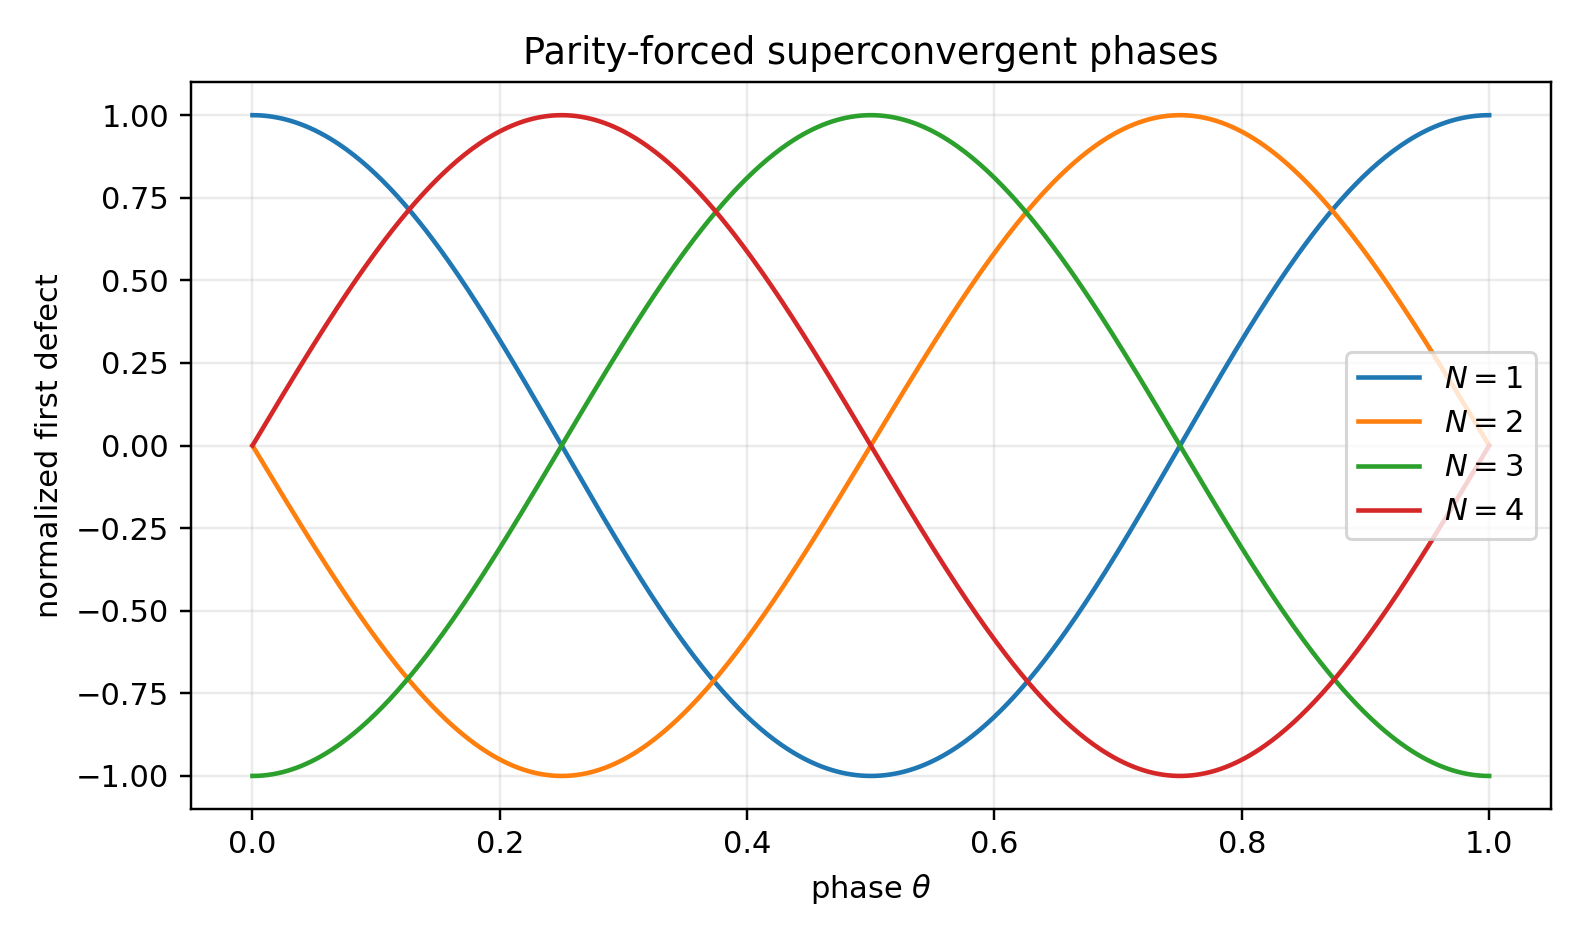
\includegraphics[width=0.88\textwidth]{defect_profiles.png}
\caption{Normalized exact first-defect profiles.  The parity-forced phases are common zeros of every odd harmonic in the corresponding sine or cosine series.}
\label{fig:defect-profiles}
\end{figure}

\subsection{A canonical phase schedule and exact experiments}

Choose
\begin{equation}
 \theta_N=
 \begin{cases}
 0,&N\ \text{even},\\
 1/4,&N\ \text{odd}.
 \end{cases}
 \label{eq:canonical-phase}
\end{equation}
Then $Q_{N,\theta_N}$ is positive, rational, and exact through degree $N+1$.  Its number of positive nodes is $2^{N+1}-1$ at centered levels and $2^{N+1}$ at quarter-shifted levels.

\begin{table}[H]
\centering
\caption{Exact rational checks of the canonical phase schedule.  ``Proved degree'' is the theorem above.  Each next defect is computed as an exact fraction; a decimal display is used here for legibility, while the full fractions are retained in the CSV and exact TeX table in the archive.}
\label{tab:quadrature-exact}
% Generated by experiments.py; exact values are in the CSV
\begin{tabular}{@{}rrrrr@{}}
\toprule
$N$ & phase $\theta_N$ & positive nodes & proved degree & next defect (decimal display)\\
\midrule
0 & $0$ & 1 & 1 & $-0.11111111$\\
1 & $1/4$ & 4 & 2 & $0.011067708$\\
2 & $0$ & 7 & 3 & $0.0002806713$\\
3 & $1/4$ & 16 & 4 & $-2.189698e-6$\\
4 & $0$ & 31 & 5 & $-4.8411566e-9$\\
5 & $1/4$ & 64 & 6 & $3.0609753e-12$\\
6 & $0$ & 127 & 7 & $5.4077218e-16$\\
7 & $1/4$ & 256 & 8 & $-2.6505694e-20$\\
8 & $0$ & 511 & 9 & $-3.5647819e-25$\\
\bottomrule
\end{tabular}

\end{table}

\begin{figure}[H]
\centering
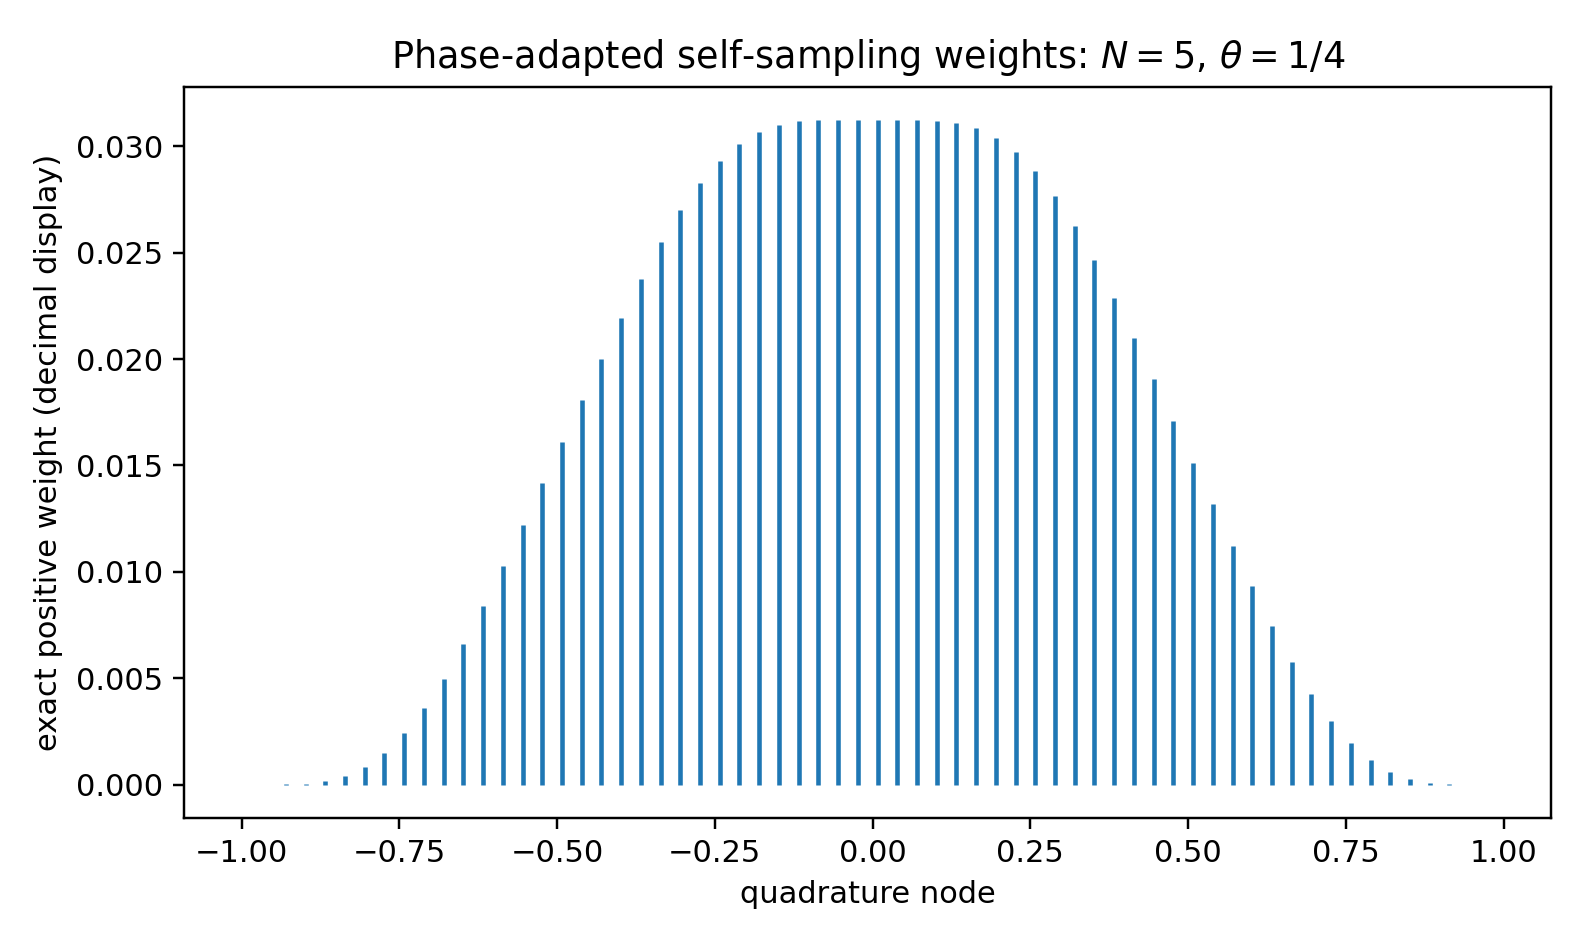
\includegraphics[width=0.88\textwidth]{quadrature_weights.png}
\caption{The positive rational weights at $N=5$, $\theta=1/4$.  The rule integrates every polynomial through degree six exactly.}
\label{fig:quadrature-weights}
\end{figure}

\begin{conjecturebox}[Exact precision conjecture]
For every $N\ge0$, the canonical rule $Q_{N,\theta_N}$ has exact degree $N+1$ and not $N+2$.  Equivalently,
\[
 E_{N,N+2}(\theta_N)\ne0
 \qquad(N\ge0).
\]
The table proves this for $0\le N\le8$ by exact rational arithmetic.  A general proof should use the two-layer decomposition $a=0,1$ in \eqref{eq:valuation-filtration} together with the Bell coefficient $\gamma_1$ in \eqref{eq:gamma1}.
\end{conjecturebox}

\section{Positive alias filters as Richardson extrapolation}
\label{sec:positive-richardson}

\subsection{Coset rules}

For $s\ge0$ and $0\le a<2^s$, define the phase-coset rule
\begin{equation}
 Q_{N;s,a}[f]
 :=2^{-N}\sum_{k\in\Z}
 f\!\left(\frac{2^sk+a}{2^{N+s}}\right)
 u\!\left(\frac{2^sk+a}{2^{N+s}}\right).
 \label{eq:coset-rule}
\end{equation}
This is simply $Q_{N,a/2^s}$, hence is positive and exact through degree $N$.

\begin{theorem}[Positive phase refinement]
\label{thm:positive-phase-refinement}
For every $s\ge0$,
\begin{equation}
 \boxed{\displaystyle
 Q_{N+s,0}[f]
 =2^{-s}\sum_{a=0}^{2^s-1}Q_{N;s,a}[f].}
 \label{eq:positive-phase-refinement}
\end{equation}
Thus averaging all $2^s$ positive phase classes gains exactly $s$ guaranteed degrees of polynomial exactness.
\end{theorem}

\begin{proof}
The integers $2^sk+a$, with $k\in\Z$ and $0\le a<2^s$, partition $\Z$.  Multiplying the outer factor $2^{-N}$ by $2^{-s}$ gives $2^{-(N+s)}$, exactly the fine-grid rule.
\end{proof}

For $s=1$, let
\[
 \nu_N=Q_{N,0},
 \qquad
 \rho_N=Q_{N,1/2}.
\]
Then
\begin{equation}
 \nu_{N+1}=\frac12(\nu_N+\rho_N),
 \qquad
 \boxed{\rho_N=2\nu_{N+1}-\nu_N.}
 \label{eq:midpoint-Richardson}
\end{equation}
The right side is the familiar signed Richardson difference, yet the left side is manifestly a positive quadrature measure.  The cancellation that is hidden in scale space becomes positivity after resolution into even and odd lattice cosets.

\subsection{Uniqueness in alias space}

Suppose coefficients $c_0,\ldots,c_{2^s-1}$ combine the phase classes.  At Fourier alias $\ell$, the multiplier is
\begin{equation}
 C(\ell)=\sum_{a=0}^{2^s-1}c_a\e^{2\pi\iu a\ell/2^s}.
 \label{eq:DFT-filter}
\end{equation}
To gain all $s$ degrees, every residue class $\ell\not\equiv0\pmod{2^s}$ must be annihilated.

\begin{theorem}[Unique full residue-class filter]
\label{thm:unique-phase-filter}
Assume
\begin{equation}
 C(0)=1,
 \qquad
 C(\ell)=0\quad(1\le\ell<2^s).
 \label{eq:DFT-conditions}
\end{equation}
Then
\begin{equation}
 c_0=c_1=\cdots=c_{2^s-1}=2^{-s}.
 \label{eq:unique-uniform-filter}
\end{equation}
Hence the positive average in \eqref{eq:positive-phase-refinement} is the unique filter on all dyadic phases that cancels every nonzero residue class modulo $2^s$.
\end{theorem}

\begin{proof}
The vector $(C(0),\ldots,C(2^s-1))$ is the discrete Fourier transform of $(c_0,\ldots,c_{2^s-1})$.  Inverting the DFT of $(1,0,\ldots,0)$ gives the uniform vector.
\end{proof}

\begin{remark}[Comparison with $q$-Richardson]
The repository's geometric Lagrange/Richardson filters cancel powers of a scale parameter and generally use signed Gaussian-$q$-binomial weights.  The filter above cancels Fourier residue classes and uses equal positive weights.  The two mechanisms act in complementary variables: scale depth versus lattice phase.  Their tensor product is a natural candidate for a stable two-parameter accelerator; see \cref{prob:hybrid-filter}.
\end{remark}

\begin{resultbox}[Third frontier bridge]
Subdividing a self-sampling rule does not merely refine a Riemann sum.  In Fourier space it applies an exact DFT projector to the alias tree.  The usual Richardson difference $2\nu_{N+1}-\nu_N$ is positive because it isolates the odd lattice coset.  This gives a rare instance in which an extrapolation operator has a hidden positive-measure realization.
\end{resultbox}

\section{Inverse-moment Rvachev--Appell polynomials}
\label{sec:appell}

\subsection{The umbral inverse of the moment family}

The frontier volume already uses the forward moment Appell sequence
\begin{equation}
 \Pcal_n(x)=\int_{-1}^{1}(x+y)^n u(y)\dd y,
 \qquad
 \sum_{n\ge0}\Pcal_n(x)\frac{z^n}{n!}=\e^{xz}M(z).
 \label{eq:forward-Appell}
\end{equation}
We now reverse the moment multiplier.

\begin{definition}[Inverse-moment Rvachev--Appell sequence]
\label{def:inverse-Appell}
Define $\Acal_n(x)$ by
\begin{equation}
 \boxed{\displaystyle
 \frac{\e^{xz}}{M(z)}
 =\sum_{n=0}^{\infty}\Acal_n(x)\frac{z^n}{n!}.}
 \label{eq:inverse-Appell-gen}
\end{equation}
\end{definition}

Because $M(0)=1$, this is a well-defined formal power series and an analytic generating function near $z=0$.  Its logarithm is
\begin{equation}
 xz-\sum_{r\ge1}\kappa_{2r}\frac{z^{2r}}{(2r)!}.
 \label{eq:inverse-Appell-log}
\end{equation}

\begin{theorem}[Bell--Bernoulli structure]
\label{thm:Appell-Bell}
The sequence $\Acal_n$ has the following properties.
\begin{enumerate}
\item It is Appell and parity adapted:
\begin{equation}
 \Acal_n'(x)=n\Acal_{n-1}(x),
 \qquad
 \Acal_n(-x)=(-1)^n\Acal_n(x).
 \label{eq:Appell-basic}
\end{equation}
\item It is a complete Bell polynomial in the Bernoulli cumulants:
\begin{equation}
 \boxed{\displaystyle
 \Acal_n(x)=Y_n(x,-\kappa_2,0,-\kappa_4,0,\ldots,-\kappa_n).}
 \label{eq:Appell-Bell}
\end{equation}
\item It satisfies the triangular recurrence
\begin{equation}
 \Acal_{n+1}(x)
 =x\Acal_n(x)
 -\sum_{j=1}^{\floor{(n+1)/2}}
 \binom n{2j-1}\kappa_{2j}\Acal_{n-2j+1}(x).
 \label{eq:Appell-recurrence}
\end{equation}
\item The forward and inverse families are umbral inverses:
\begin{equation}
 M(D)\Acal_n(x)=x^n,
 \qquad
 M(D)^{-1}\Pcal_n(x)=x^n,
 \qquad D=\frac{\dd}{\dd x}.
 \label{eq:umbral-inverse}
\end{equation}
\end{enumerate}
\end{theorem}

\begin{proof}
Differentiate \eqref{eq:inverse-Appell-gen} with respect to $x$ for the Appell law; use the evenness of $M$ for parity.  Equation \eqref{eq:Appell-Bell} is the defining generating identity of complete exponential Bell polynomials applied to \eqref{eq:inverse-Appell-log}.  Differentiating with respect to $z$ gives
\[
 \frac{\partial}{\partial z}\frac{\e^{xz}}{M(z)}
 =\left(x-\frac{M'(z)}{M(z)}\right)\frac{\e^{xz}}{M(z)},
\]
and coefficient comparison gives \eqref{eq:Appell-recurrence}.  Finally, $M(D)$ multiplies an exponential $\e^{xz}$ by $M(z)$, proving \eqref{eq:umbral-inverse} on exponential generating functions.
\end{proof}

The first polynomials are reproduced in \cref{app:Appell-table}.  In compact notation,
\begin{align*}
 \Acal_2(x)&=x^2-\frac19,\\
 \Acal_4(x)&=x^4-\frac23x^2+\frac{31}{675},\\
 \Acal_6(x)&=x^6-\frac53x^4+\frac{31}{45}x^2-\frac{2347}{59535}.
\end{align*}
The constants are the signed complete Bell transforms of the rational cumulants; no transcendental constants remain.

\subsection{Continuous deconvolution}

\begin{theorem}[Exact deconvolution identity]
\label{thm:Appell-deconvolution}
For every $n\ge0$ and $x\in\R$,
\begin{equation}
 \boxed{\displaystyle
 \int_{-1}^{1}\Acal_n(x-y)u(y)\dd y=x^n.}
 \label{eq:Appell-deconvolution}
\end{equation}
Equivalently, the convolution operator by $u$ maps the inverse-moment Appell basis to the monomial basis.
\end{theorem}

\begin{proof}
Multiply generating functions:
\begin{align*}
 \int_{-1}^{1}\frac{\e^{(x-y)z}}{M(z)}u(y)\dd y
 &=\frac{\e^{xz}}{M(z)}M(-z)\\
 &=\e^{xz},
\end{align*}
using the evenness $M(-z)=M(z)$.  Compare coefficients of $z^n/n!$.
\end{proof}

\begin{corollary}[Mean-zero Appell cancellations]
\label{cor:Appell-mean-zero}
For $n\ge1$,
\begin{equation}
 \int_{-1}^{1}\Acal_n(x)u(x)\dd x=0.
 \label{eq:Appell-mean-zero}
\end{equation}
\end{corollary}

\begin{proof}
Set $x=0$ in \eqref{eq:Appell-deconvolution} and use parity.
\end{proof}

\subsection{Finite lattice reproduction}

The self-sampling theorem discretizes the deconvolution identity without loss.

\begin{theorem}[Finite Rvachev--Appell translation formula]
\label{thm:Appell-lattice-reproduction}
Let $N\ge0$, $\theta\in\R$, and $0\le n\le N$.  Then, for every $x\in\R$,
\begin{equation}
 \boxed{\displaystyle
 x^n=2^{-N}\sum_{k\in\Z}
 \Acal_n\!\left(x-\frac{k+\theta}{2^N}\right)
 u\!\left(\frac{k+\theta}{2^N}\right).}
 \label{eq:Appell-lattice-reproduction}
\end{equation}
The sum is finite.  At a superconvergent phase from \cref{cor:forced-superconvergence}, the identity remains valid for $n=N+1$.
\end{theorem}

\begin{proof}
For fixed $x$, the map $y\mapsto\Acal_n(x-y)$ is a polynomial of degree $n$.  Apply \cref{thm:self-sampling} to the integral in \eqref{eq:Appell-deconvolution}.
\end{proof}

More generally, for a polynomial $p$ define its Rvachev deconvolution
\begin{equation}
 \mathscr D_up
 :=M(D)^{-1}p
 =\exp\!\left(-\sum_{r\ge1}\kappa_{2r}
 \frac{D^{2r}}{(2r)!}\right)p.
 \label{eq:polynomial-deconvolution}
\end{equation}
The exponential truncates because $p$ is a polynomial.

\begin{corollary}[Polynomial reproduction by deconvolved translates]
\label{cor:polynomial-deconvolution}
If $\deg p\le N$, then
\begin{equation}
 p(x)=2^{-N}\sum_{k\in\Z}
 (\mathscr D_up)\!\left(x-\frac{k+\theta}{2^N}\right)
 u\!\left(\frac{k+\theta}{2^N}\right).
 \label{eq:general-deconvolution-reproduction}
\end{equation}
\end{corollary}

\begin{resultbox}[Fourth frontier bridge]
The forward moment Appell family packages convolution by the up-law; the reciprocal family $\Acal_n$ packages deconvolution.  The same positive dyadic samples that integrate ordinary polynomials now reproduce ordinary monomials from translates of $\Acal_n$.  This simultaneously connects the Fourier zeros, Bernoulli cumulants, complete Bell polynomials, and finite rational Fabius values.
\end{resultbox}

\subsection{Root geometry: an exact counterexample to real-rootedness}

The first seven polynomials have only real zeros numerically, which makes global real-rootedness a tempting conjecture.  It fails immediately afterward.

\begin{proposition}[First certified nonreal zeros]
\label{prop:A8-roots}
The exact polynomial
\begin{equation}
 \Acal_8(x)
 =x^8-\frac{28}{9}x^6+\frac{434}{135}x^4
 -\frac{9388}{8505}x^2+\frac{1904369}{32531625}
 \label{eq:A8}
\end{equation}
has exactly four real zeros.  Hence its other four zeros are nonreal and form two conjugate pairs.
\end{proposition}

\begin{proof}[Computer-assisted exact proof]
The coefficients lie in $\Q$.  The accompanying script constructs the exact polynomial in $\Q[x]$ from \eqref{eq:Appell-recurrence} and applies a Sturm sequence on $(-\infty,\infty)$.  The exact sign-variation count is four.  No floating-point root classification enters this count.  The certificate and source are included in the archive.
\end{proof}

\begin{figure}[H]
\centering
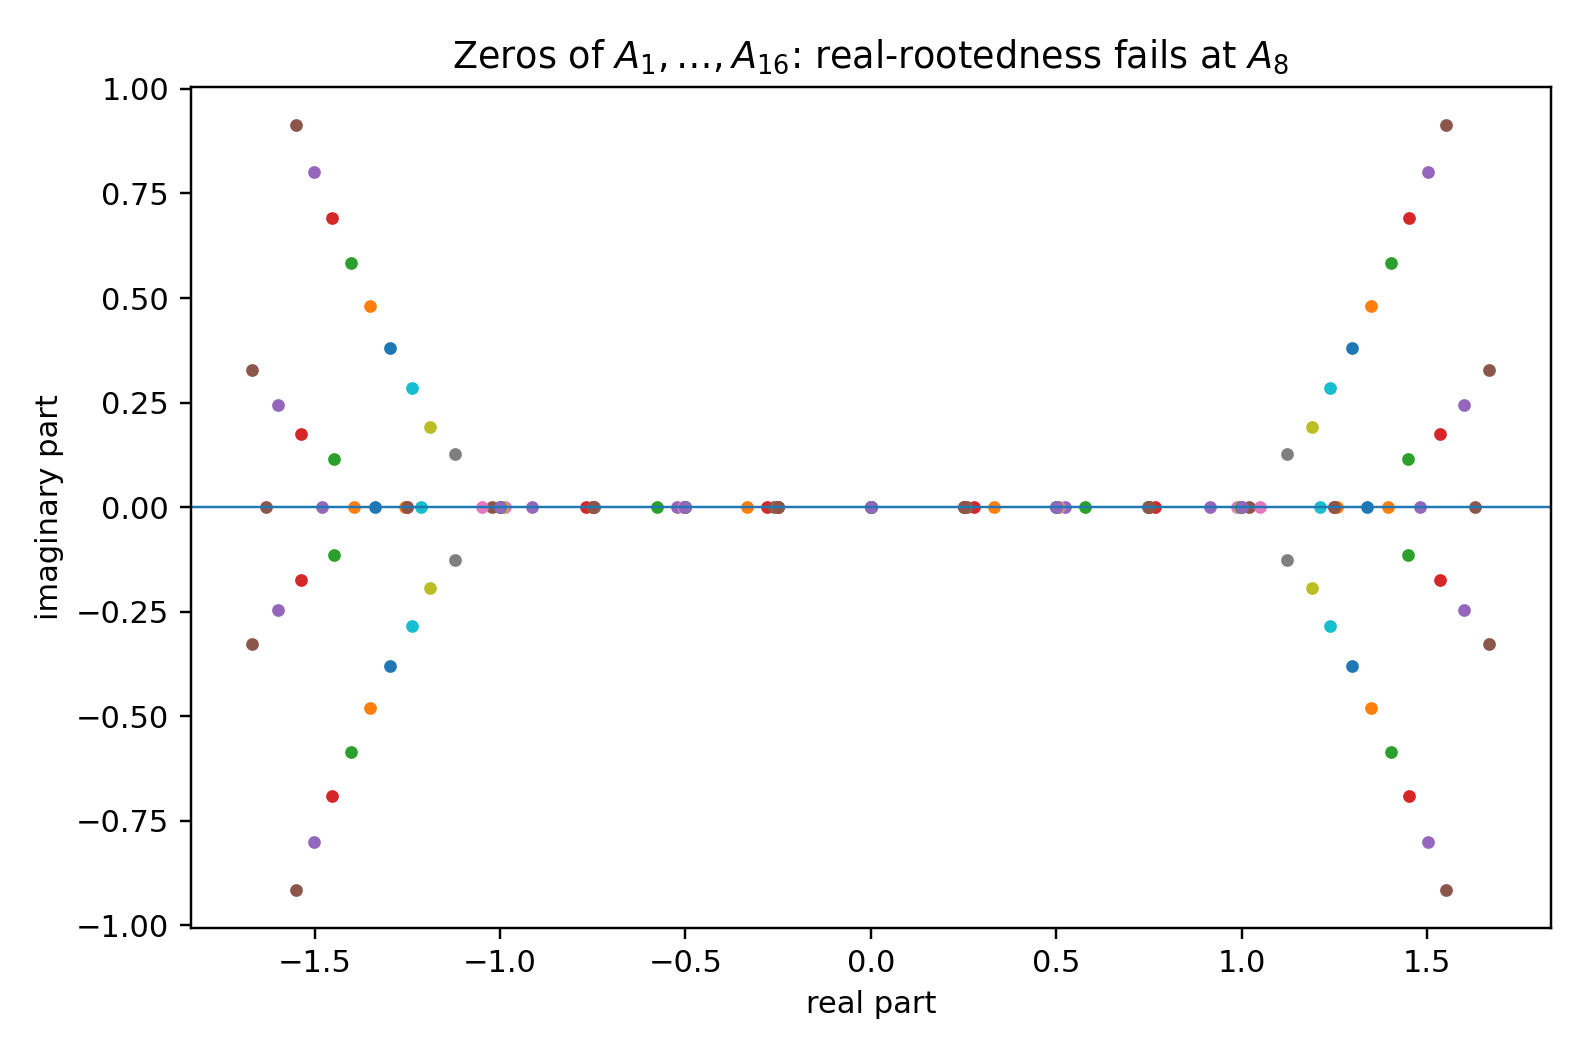
\includegraphics[width=0.86\textwidth]{appell_roots.png}
\caption{Numerical locations of the zeros of $\Acal_1,\ldots,\Acal_{16}$.  The exact Sturm result certifies the first departure from the real axis at degree eight; the later pattern is exploratory.}
\label{fig:Appell-roots}
\end{figure}

The computed nonreal-root counts through degree $30$ are
\begin{center}
\begin{tabular}{@{}lrrrrrr@{}}
\toprule
Degree range & $1$--$7$ & $8$--$12$ & $13$--$17$ & $18$--$22$ & $23$--$28$ & $29$--$30$\\
\midrule
Nonreal roots & $0$ & $4$ & $8$ & $12$ & $16$ & $20$\\
\bottomrule
\end{tabular}
\end{center}
This staircase is not asserted as a theorem; it motivates \cref{conj:Appell-root-staircase}.

\section{Transport through the inverse Fabius function}
\label{sec:inverse-transport}

The centered quantile $q(t)=2F^{-1}(t)-1$ pushes Lebesgue measure on $[0,1]$ to the up-law.  Therefore
\begin{equation}
 \int_0^1g(q(t))\dd t=\int_{-1}^{1}g(x)u(x)\dd x
 \label{eq:quantile-transport}
\end{equation}
for every bounded Borel function $g$.

\begin{theorem}[Rational inverse-Fabius quadrature]
\label{thm:inverse-Fabius-quadrature}
Let $\theta=a/2^s$ and retain the dyadic nodes $x_k=n_k/2^D$ and weights $w_k$ from \cref{cor:rational-rules}.  Define
\begin{equation}
 t_k=F\!\left(\frac{1+x_k}{2}\right)\in\Q.
 \label{eq:inverse-Fabius-nodes}
\end{equation}
Then $q(t_k)=x_k$, and for every polynomial $p$ with $\deg p\le N$,
\begin{equation}
 \boxed{\displaystyle
 \int_0^1p\bigl(2F^{-1}(t)-1\bigr)\dd t
 =\sum_k w_k\,p\bigl(2F^{-1}(t_k)-1\bigr)
 =\sum_k w_kp(x_k).}
 \label{eq:inverse-Fabius-quadrature}
\end{equation}
At a phase-superconvergent level the exactness extends to $\deg p\le N+1$.
\end{theorem}

\begin{proof}
Equation \eqref{eq:centered-CDF} implies $q(t_k)=x_k$.  Apply \eqref{eq:quantile-transport} and then \cref{thm:self-sampling}.  Rationality follows because both $(1+x_k)/2$ and the weight arguments are dyadic.
\end{proof}

\begin{remark}[A nonlinear exactness space]
The rule in \eqref{eq:inverse-Fabius-quadrature} is not claimed to integrate all ordinary polynomials in $t$.  It integrates exactly the non-elementary space
\begin{equation}
 \mathcal V_N
 =\operatorname{span}\{1,q(t),q(t)^2,\ldots,q(t)^N\},
 \qquad q(t)=2F^{-1}(t)-1,
 \label{eq:inverse-exactness-space}
\end{equation}
using rational nodes $t_k$, rational weights $w_k$, and no numerical inversion.  This is an exact finite interface between the inverse Fabius function and dyadic arithmetic.
\end{remark}

\subsection{Endpoint nodes and the Lambert coordinate}

For centered rules, the smallest nonzero endpoint distance is $2^{-N}$ and the corresponding extreme weights are
\begin{equation}
 2^{-N}F(2^{-N}).
 \label{eq:centered-extreme-weight}
\end{equation}
For quarter-shifted rules, the leftmost distance is $2^{-N-2}$, so one extreme weight is
\begin{equation}
 2^{-N}F(2^{-N-2}).
 \label{eq:quarter-extreme-weight}
\end{equation}
The corpus's sharp endpoint theory expresses $F(x)$ through the exact lower-Lambert coordinate
\begin{equation}
 \lambda(x)=-\frac1{\log2}W_{-1}(-x\log2),
 \qquad x=\lambda2^{-\lambda},
 \label{eq:Lambert-coordinate}
\end{equation}
with a nonconstant periodic correction in the dyadic phase of $\lambda$.  Thus the new quadrature rules supply exact rational global moment constraints whose smallest weights lie precisely in the Lambert boundary layer.  Turning these constraints into identities for the endpoint periodic factor is an open program formulated in \cref{prob:Lambert-sum-rules}.

\section{Finite Gaussian-$q$-binomial identities forced by quadrature}
\label{sec:qbinomial}

\subsection{The exact dyadic evaluator}

Let
\begin{equation}
 (q;q)_n=\prod_{j=1}^{n}(1-q^j),
 \qquad
 \qbinom{n}{k}{q}=\frac{(q;q)_n}{(q;q)_k(q;q)_{n-k}}.
 \label{eq:q-notation-report}
\end{equation}
For integers $m,n\ge0$ and $c\in\Q$, define
\begin{equation}
\begin{aligned}
 \mathfrak Q_n(m;c)
 :={}&\frac{1}{2^{n^2}(1/2;1/2)_n}
 \sum_{j=0}^{n}
 \frac{\qbinom{n}{j}{1/2}}
      {2^{j(j-1)}(n+j)!}\\
 &\qquad\times
 \sum_{r=0}^{m2^j-1}\eps_r
 \bigl(r-m2^j+c\bigr)^{n+j}.
 \label{eq:Qfrak-def}
\end{aligned}
\end{equation}
The established arbitrary-numerator theorem states
\begin{equation}
 \mathfrak Q_n(m;c)=F(m/2^n)
 \qquad(0\le m\le2^n),
 \label{eq:Qfrak-F}
\end{equation}
and the right side of \eqref{eq:Qfrak-def} is independent of $c$.  Its Gaussian coefficients arise from Lagrange interpolation on a geometric grid.

\subsection{A $q$-binomial--Thue--Morse--Bell identity}

\begin{theorem}[Finite arithmetic moment identity]
\label{thm:qbinomial-moment-identity}
Let $\theta=a/2^s$, $D=N+s$, $n_k=2^sk+a$, and $b_k=2^D-\abs{n_k}$.  For every $0\le r\le N$ and every $c\in\Q$,
\begin{equation}
 \boxed{\displaystyle
 \mu_r
 =2^{-N-Dr}
 \sum_{\abs{n_k}<2^D}
 n_k^r\,\mathfrak Q_D(b_k;c).}
 \label{eq:qbinomial-moment-identity}
\end{equation}
At the superconvergent phases of \cref{cor:forced-superconvergence}, the identity also holds for $r=N+1$.  Therefore the finite Gaussian-$q$-binomial--Thue--Morse sum on the right equals
\begin{equation}
 Y_r(0,\kappa_2,0,\kappa_4,\ldots,\kappa_r),
 \label{eq:qbinomial-Bell-right}
\end{equation}
where the cumulants are the Bernoulli rationals in \eqref{eq:cumulants}.
\end{theorem}

\begin{proof}
At node $x_k=n_k/2^D$, \eqref{eq:F-up-relation} and \eqref{eq:Qfrak-F} give
\[
 u(x_k)=F(b_k/2^D)=\mathfrak Q_D(b_k;c).
\]
Substitute this into \eqref{eq:self-sampling-main}, then use \eqref{eq:moment-Bell}.
\end{proof}

\begin{remark}[Why this identity is structurally new]
Each ingredient existed separately: the $q$-binomial evaluator, the Bell moment formula, and the zero multiplicities.  The self-sampling theorem forces them into a single positive finite identity.  The common translation $c$ disappears after a double finite summation, giving a family of nontrivial translation-invariance identities among Thue--Morse power sums.
\end{remark}

\begin{corollary}[Finite Appell cancellation in $q$-arithmetic]
\label{cor:q-Appell-cancellation}
For $1\le n\le N$,
\begin{equation}
 \sum_{\abs{n_k}<2^D}
 \Acal_n\!\left(-\frac{n_k}{2^D}\right)
 \mathfrak Q_D(b_k;c)=0.
 \label{eq:q-Appell-cancellation}
\end{equation}
After inserting \eqref{eq:Qfrak-def}, this is a finite identity containing Gaussian $q$-binomial coefficients, Thue--Morse signs, Bernoulli cumulants, and complete Bell polynomials.
\end{corollary}

\begin{proof}
Set $x=0$ in \eqref{eq:Appell-lattice-reproduction} and clear the common factor $2^{-N}$.
\end{proof}

\section{Base-$b$ and multidimensional extensions}
\label{sec:extensions}

\subsection{Integer dilation bases}

Let $b\ge2$ be an integer and define
\begin{equation}
 \Phi_b(\xi)=\prod_{j=0}^{\infty}
 \sincpi\!\left(\frac{\xi}{b^j}\right).
 \label{eq:Phi-b}
\end{equation}
It is the characteristic function of a compactly supported smooth probability density $u_b$, obtained as an infinite convolution of centered uniform laws.  The support radius is $b/(2(b-1))$.

If $m\ne0$ is an integer, then
\begin{equation}
 \ord_{\xi=m}\Phi_b=1+\nu_b(m),
 \label{eq:b-multiplicity}
\end{equation}
where $\nu_b(m)$ is the largest $a$ such that $b^a\mid m$.

\begin{theorem}[Base-$b$ self-sampling]
\label{thm:base-b}
For every $N\ge0$, phase $\theta$, and polynomial $p$ of degree at most $N$,
\begin{equation}
 \int p(x)u_b(x)\dd x
 =b^{-N}\sum_{k\in\Z}
 p\!\left(\frac{k+\theta}{b^N}\right)
 u_b\!\left(\frac{k+\theta}{b^N}\right).
 \label{eq:base-b-self-sampling}
\end{equation}
Moreover, averaging the $b^s$ phases $a/b^s$ gives the level-$N+s$ rule and is the unique full DFT filter annihilating every nonzero residue modulo $b^s$.
\end{theorem}

\begin{proof}
Repeat the Poisson argument.  A nonzero alias $b^N\ell$ has zero order $N+1+\nu_b(\ell)$.  The coset and uniqueness arguments are identical with the $b^s$-point DFT.
\end{proof}

The binary case is distinguished arithmetically because half-integer spectral signs reduce to the classical Thue--Morse sequence and dyadic Fabius values are rational.  For general $b$, the same analytic framework suggests generalized digital sign sequences and $q=b^{-1}$ arithmetic.

\subsection{Tensor-product cubature}

Let
\begin{equation}
 U_d(x_1,\ldots,x_d)=\prod_{j=1}^{d}u(x_j).
 \label{eq:tensor-density}
\end{equation}
Tensoring \cref{thm:self-sampling} gives a positive cubature rule.

\begin{corollary}[Positive tensor cubature]
\label{cor:tensor-cubature}
For a polynomial $p$ whose degree in each coordinate is at most $N$,
\begin{equation}
 \int_{[-1,1]^d}p(\bm x)U_d(\bm x)\dd\bm x
 =2^{-Nd}\sum_{\bm k\in\Z^d}
 p\!\left(\frac{\bm k+\bm\theta}{2^N}\right)
 U_d\!\left(\frac{\bm k+\bm\theta}{2^N}\right).
 \label{eq:tensor-cubature}
\end{equation}
The sum is finite and positive.  Coordinatewise phase superconvergence raises the exactness by one in every selected coordinate.
\end{corollary}

The node count grows exponentially with $d$, so sparse-grid combinations and hyperbolic-cross alias filters are a natural next step; see \cref{prob:sparse-grid}.

\section{Exact and high-precision experiments}
\label{sec:experiments}

The numerical work was designed to test formulas only after they had been derived.  Exact rational arithmetic is used for moments, dyadic Fabius values, quadrature weights, and finite defects.  High-precision floating-point arithmetic is used only for the infinite Fourier products and figures.  Symbolic polynomial arithmetic over $\Q$ is used for the Appell sequence and the Sturm root count.

\subsection{Independent check of the spectral defect}

At the generic dyadic phase $\theta=1/8$, neither parity family is forced to vanish.  For each $0\le N\le7$, the script computes
\[
 Q_{N,1/8}[x^{N+1}]-\mu_{N+1}
\]
exactly from rational Fabius values, and independently evaluates the series in \eqref{eq:first-defect-complex} at 90 decimal digits.

\begin{table}[H]
\centering
\caption{Independent exact-versus-spectral verification at $\theta=1/8$.  The first numerical column is obtained from exact rational arithmetic and displayed decimally; the full fractions are retained in the archive.}
\label{tab:spectral-check}
% Generated by experiments.py at 90 decimal digits
\begin{tabular}{@{}rrrr@{}}
\toprule
$N$ & exact defect (decimal) & spectral series & absolute difference\\
\midrule
0 & $0.121527777778$ & $0.121527777778$ & $2.62e-21$\\
1 & $0.0100171199846$ & $0.0100171199846$ & $2.89e-24$\\
2 & $-0.000295110631872$ & $-0.000295110631872$ & $3.27e-29$\\
3 & $-2.9473755642e-6$ & $-2.9473755642e-6$ & $3.92e-33$\\
4 & $9.14914262587e-9$ & $9.14914262587e-9$ & $5.29e-39$\\
5 & $8.5358933664e-12$ & $8.5358933664e-12$ & $4.92e-44$\\
6 & $-2.32134975825e-15$ & $-2.32134975825e-15$ & $7.03e-51$\\
7 & $-1.80406749858e-19$ & $-1.80406749858e-19$ & $4.21e-57$\\
\bottomrule
\end{tabular}

\end{table}

The residual decreases as more spectral terms become negligible; the displayed discrepancies are truncation errors, not fitted residuals.

\subsection{Exact arithmetic workflow}

The main exact evaluator implements \eqref{eq:finite-F-moment} literally.  A representative excerpt is:

\begin{lstlisting}[style=frontiercode,caption={Exact dyadic Fabius evaluation and shifted moment quadrature.}]
@lru_cache(maxsize=None)
def fabius_dyadic(a: int, n: int) -> Fraction:
    moments = even_moments(n // 2)
    outer = Fraction(0)
    for h in range(a):
        inner = Fraction(0)
        for k in range(n // 2 + 1):
            inner += (Fraction(comb(n, 2*k))
                      * (2*a - 2*h - 1)**(n - 2*k)
                      * moments[k])
        outer += thue_morse_sign(h) * inner
    return outer / (factorial(n) * 2**(n*(n + 1)//2))


def shifted_quadrature_moment(N, degree, a=0, s=0):
    D = N + s
    total = Fraction(0)
    for k in range(-2**N - 2, 2**N + 3):
        numerator = 2**s * k + a
        if abs(numerator) < 2**D:
            x = Fraction(numerator, 2**D)
            total += (Fraction(1, 2**N)
                      * up_dyadic(numerator, D) * x**degree)
    return total
\end{lstlisting}

For every row of \cref{tab:quadrature-exact}, the program first asserts all claimed moment identities exactly and only then writes the next nonzero defect.  The complete, heavily commented script is included in the archive.

\subsection{Reproducibility boundary}

The following distinction is essential:
\begin{itemize}
\item \cref{thm:self-sampling,thm:master-alias,thm:first-defect,thm:Bernoulli-convolution,thm:phase-classification,thm:positive-phase-refinement,thm:Appell-deconvolution,thm:Appell-lattice-reproduction,thm:qbinomial-moment-identity} are proved analytically in the text;
\item the rational tables verify special cases but are not used as proofs of the general identities;
\item \cref{prop:A8-roots} uses an exact computer algebra proof via Sturm's theorem;
\item the root counts beyond degree eight and all plotted root locations are exploratory numerical evidence.
\end{itemize}

\section{Conjectures and frontier research program}
\label{sec:frontier}

\subsection{The next alias layer}

\begin{conjecture}[Exact phase-adapted precision and sign]
\label{conj:next-defect-sign}
Let $\theta_N$ be the canonical phase in \eqref{eq:canonical-phase}.  Then
\begin{equation}
 E_{N,N+2}(\theta_N)\ne0
 \qquad(N\ge0).
 \label{eq:next-defect-nonzero}
\end{equation}
Moreover, for $N\ge1$, the experimental sign law is
\begin{equation}
 \sgn E_{N,N+2}(\theta_N)
 =(-1)^{\floor{(N-1)/2}}.
 \label{eq:next-defect-sign-conj}
\end{equation}
\end{conjecture}

The exact two-layer formula is given in \cref{app:next-defect}.  A proof should combine:
\begin{enumerate}
\item the odd-alias contribution with one Bell correction $\gamma_1$;
\item the twice-odd contribution with its leading zero jet;
\item the parity-specific phase factors;
\item a first-frequency dominance estimate sharp enough to control the logarithmic derivative $\Phi'/\Phi$ at half-integers.
\end{enumerate}
A successful argument would determine the exact degree of every positive phase-adapted rule.

\begin{problem}[All higher phase gains]
\label{prob:higher-phase-gains}
For fixed excess $s\ge2$, classify all phases $\theta$ for which
\[
 E_{N,N+1}(\theta)=\cdots=E_{N,N+s}(\theta)=0.
\]
The valuation filtration makes this a finite hierarchy of trigonometric equations built from alias layers $0,\ldots,s-1$.  Determine whether any single positive phase can gain more than one degree for infinitely many $N$.
\end{problem}

\subsection{Optimal phase and scale filters}

\begin{problem}[Hybrid DFT--Gaussian-$q$ filter]
\label{prob:hybrid-filter}
Combine the positive DFT projector in \eqref{eq:positive-phase-refinement} with the repository's geometric Gaussian-$q$-binomial Richardson filters in the scale variable.  For a prescribed exactness order, minimize:
\begin{enumerate}
\item total variation of the combined coefficients;
\item number of distinct dyadic Fabius evaluations;
\item largest denominator of an exact rational coefficient;
\item sensitivity near the flat endpoints.
\end{enumerate}
A two-stage construction may first remove low $2$-adic alias classes by positive phase averaging and then remove the remaining scale modes by a short signed $q$-Richardson filter.
\end{problem}

\begin{conjecture}[Positive extremality]
\label{conj:positive-extremality}
Among combinations of all $2^s$ dyadic phase classes that gain $s$ degrees uniformly for every level $N$, the uniform average is not only unique under exact residue annihilation, as proved in \cref{thm:unique-phase-filter}, but also minimizes every convex coefficient cost, including $\ell^p$ norms and entropy penalties.
\end{conjecture}

The uniqueness theorem makes this plausible for the full filter.  A subtler variant allows only selected residue classes or allows level-dependent approximate cancellation; then nonuniform positive designs may exist.

\subsection{Denominators and arithmetic geometry}

\begin{problem}[Exact valuations of self-sampling weights]
\label{prob:weight-valuations}
For dyadic $\theta=a/2^s$, determine the exact prime valuations of
\[
 w_{N,\theta,k}=2^{-N}F\!\left(1-\frac{\abs{2^sk+a}}{2^{N+s}}\right)
\]
in lowest terms.  Natural targets are:
\begin{enumerate}
\item exact $2$-adic valuations of the extreme weights;
\item odd-prime divisibility controlled by Mersenne factors $2^{2j}-1$;
\item the least common denominator of the complete rule;
\item cancellation in the rational next defect $E_{N,N+2}(\theta_N)$.
\end{enumerate}
The q-binomial identity \eqref{eq:qbinomial-moment-identity} supplies a second route to the same valuations and may reveal cancellations invisible in the moment formula.
\end{problem}

\begin{conjecture}[Primitive normalized phase rules]
\label{conj:primitive-rules}
After clearing the established common denominator at level $D=N+s$, the integer weight vector of a primitive dyadic phase has greatest common divisor one, except for explicitly classifiable symmetries caused by dyadic refinement.
\end{conjecture}

\subsection{Rvachev--Appell zero geometry}

\begin{conjecture}[Unbounded nonreal root count]
\label{conj:Appell-root-staircase}
The number of nonreal zeros of $\Acal_n$ tends to infinity with $n$.  After scaling $x=n\zeta/(2\pi)$, the zero counting measures converge to a deterministic compact set governed by the nearest poles $z=\pm2\pi\iu$ of $1/M(z)$ and by the dyadic multiplicity hierarchy at $z=\pm2^{j+1}\pi\iu$.
\end{conjecture}

This conjecture is more cautious than extrapolating the short staircase in the data.  General asymptotic theory for Appell polynomials with meromorphic generating functions suggests that the nearest singularities control the zero attractor, but the repeated dyadic pole multiplicities should create nonstandard transitions.

\begin{problem}[A spectral asymptotic for $\Acal_n$]
\label{prob:Appell-spectral-asymptotic}
Use residues of $\e^{xz}/M(z)$ to derive an expansion for $\Acal_n(x)/n!$ that is uniform in the zero-scaling regime.  Determine:
\begin{enumerate}
\item the first curve on which the contributions from $\pm2\pi\iu$ balance;
\item how the next dyadic poles perturb that curve;
\item whether the observed root-count plateaus have an exact spectral explanation;
\item whether a Jensen-polynomial or multiplier-sequence normalization restores real-rootedness.
\end{enumerate}
\end{problem}

\subsection{Lambert endpoint sum rules}

\begin{problem}[Exact quadrature constraints on the periodic endpoint factor]
\label{prob:Lambert-sum-rules}
Insert the repository's all-orders endpoint expansion for $F(x)$, written in the lower-Lambert coordinate \eqref{eq:Lambert-coordinate}, into the exact identities \eqref{eq:centered-moment-F} and \eqref{eq:qbinomial-moment-identity}.  After separating the bulk from a shrinking endpoint boundary layer, derive explicit linear or nonlinear sum rules for the periodic coefficient functions.
\end{problem}

The principal difficulty is uniformity: the number of dyadic samples grows with $N$, while the Lambert expansion is strongest only near the endpoints.  A viable strategy is to choose a cutoff $j\le J(N)$, use the endpoint transseries on that range, and control the remaining samples by smooth quadrature estimates.  Exactness of the full moment identity should force cancellation between the two endpoint layers and the bulk.

\begin{conjecture}[Phase locking of extreme quantile nodes]
\label{conj:quantile-phase-locking}
For the inverse-Fabius quadrature in \eqref{eq:inverse-Fabius-quadrature}, the extreme rational nodes $t_k$ admit a lower-Lambert expansion whose log-periodic phase is locked to the parity schedule \eqref{eq:canonical-phase}.  After the leading endpoint terms are removed, a two-level phase-Richardson combination has an error smaller by a full inverse-Lambert order.
\end{conjecture}

This is deliberately stated as a research conjecture.  The repository already develops inverse-Fabius Lambert--Bell asymptotics; the new question is how those expansions interact with the exact positive moment designs.

\subsection{Digital generalizations and higher dimensions}

\begin{problem}[Base-$b$ spectral signs]
\label{prob:base-b-signs}
For the product \eqref{eq:Phi-b}, determine the sign and phase of $\Phi_b((bk+r)/b)$ on each nonzero residue class $r$.  Identify the resulting automatic sequence and its analogues of Prouhet cancellation, Mahler equations, and $q$-binomial arithmetic.
\end{problem}

\begin{problem}[Sparse-grid Rvachev cubature]
\label{prob:sparse-grid}
Construct Smolyak or hyperbolic-cross combinations of the tensor rules \eqref{eq:tensor-cubature} that preserve as much positivity as possible.  The alias description suggests indexing components by $2$-adic valuation vectors rather than by total scale alone.  Determine optimal node counts for coordinatewise or total-degree exactness.
\end{problem}

\begin{problem}[Nonproduct Rvachev laws]
\label{prob:nonproduct-laws}
Replace the tensor product by compactly supported refinable densities associated with a dilation matrix.  Characterize when Fourier zero multiplicities on the dual lattice make the density's own samples into a positive polynomial cubature rule.
\end{problem}

\section{Lean formalization roadmap}
\label{sec:lean}

The new results divide naturally into four tiers.

\subsection{Tier I: finite arithmetic and Appell algebra}

This tier avoids Fourier analysis and can begin immediately from the existing exact evaluator.
\begin{enumerate}[label=\textbf{I.\arabic*}]
\item Define $\Acal_n$ by the recurrence \eqref{eq:Appell-recurrence} over $\Q[x]$.
\item Prove parity, derivative, and the Bell-polynomial coefficient formula.
\item Verify the explicit polynomials through a chosen degree by reflection.
\item Formalize the exact rational tables in \cref{tab:quadrature-exact} as executable examples, not as substitutes for the analytic theorem.
\item Prove the finite q-binomial substitution identity once self-sampling is available.
\end{enumerate}
Candidate theorem names include
\begin{center}
\begin{minipage}{0.86\textwidth}\small\ttfamily
rvachevAppell\_deriv\\
rvachevAppell\_parity\\
rvachevAppell\_eq\_bell\\
rvachevAppell\_recurrence
\end{minipage}
\end{center}

\subsection{Tier II: Fourier zeros and Poisson summation}

The core analytic theorem requires reusable infrastructure:
\begin{enumerate}[label=\textbf{II.\arabic*}]
\item the infinite sinc product as the Fourier transform of the up density;
\item exact order of the zero at every nonzero integer;
\item shifted Poisson summation for $C_c^\infty$ functions;
\item the derivative-transform identity for $x^ru(x)$;
\item termwise differentiation of the master alias series.
\end{enumerate}
The target statements are
\begin{center}
\begin{minipage}{0.86\textwidth}\small\ttfamily
upSelfSampling\_monomial\\
upSelfSampling\_polynomial\\
upAliasGeneratingFunction\\
upMomentDefect\_valuationSupport
\end{minipage}
\end{center}

\subsection{Tier III: first defect and superconvergence}

Once the analytic layer is in place, formalize:
\begin{enumerate}[label=\textbf{III.\arabic*}]
\item the exact local factorization \eqref{eq:local-factorization};
\item the leading zero jet \eqref{eq:first-zero-jet};
\item the half-integer Thue--Morse sign law;
\item the periodic Bernoulli convolution identity;
\item the elementary lower bound $\Phi(1/2)>4/9$;
\item the trigonometric factor bounds and exact phase classification.
\end{enumerate}
The Bernoulli convolution may be postponed if periodic distributions are expensive; the sine/cosine series already suffices for superconvergence.

\subsection{Tier IV: probability transport and positive filters}

The final tier is largely algebraic once self-sampling is proved:
\begin{enumerate}[label=\textbf{IV.\arabic*}]
\item positivity and rationality of dyadic weights;
\item phase-coset refinement and DFT uniqueness;
\item Appell deconvolution by formal generating functions;
\item finite Appell translation reproduction;
\item inverse-Fabius transport using the quantile pushforward;
\item base-$b$ and tensor-product generalizations.
\end{enumerate}

\begin{statusbox}[Recommended first formalization target]
The best compact target is the chain
\[
 \texttt{integer zero order}
 \Longrightarrow
 \texttt{self-sampling monomials}
 \Longrightarrow
 \texttt{phase superconvergence}.
\]
It gives a new theorem with a short conceptual proof and reuses Fourier infrastructure already central to the formal development.  The inverse-moment Appell recurrence can be formalized independently in parallel.
\end{statusbox}

\section{Conclusion}
\label{sec:conclusion}

The dyadic sinc product contains a quadrature rule that is easy to overlook because its nodes and weights are made from the same function.  At mesh $2^{-N}$, every shifted lattice samples the up density into a positive probability measure matching the first $N$ moments exactly.  The proof is one line after the right normalization is chosen: the nonzero Poisson aliases land at integer zeros of multiplicity at least $N+1$.

The first failure is considerably richer.  It is simultaneously
\begin{enumerate}
\item a derivative of the infinite sinc product at its integer zero divisor;
\item a half-integer spectral Dirichlet series with Thue--Morse signs;
\item an exact periodic convolution of a Bernoulli polynomial with a rescaled up-kernel;
\item a parity-sensitive trigonometric function whose only zeros, from level two onward, give the unique phase-superconvergent positive rules.
\end{enumerate}
This four-way identity turns Fourier arithmetic into a practical design principle: centered phases are optimal at even levels, quarter phases at odd levels, and full phase averages implement positive Richardson extrapolation by projecting away alias residue classes.

The reciprocal moment generating function contributes a second new structure.  Its Appell polynomials have rational Bell--Bernoulli coefficients, deconvolve the up-law, and are reproduced exactly by the finite self-sampling measures.  Their root geometry is already nonclassical: exact Sturm arithmetic proves that real-rootedness fails at degree eight.  Substitution of the Gaussian-$q$-binomial dyadic evaluator then converts the analytic quadrature theorem into finite identities involving Lagrange weights, $q$-Pochhammer factors, Thue--Morse power sums, Bernoulli cumulants, and Bell polynomials.

The most promising next steps are now sharply posed: prove the exact next-defect sign, determine denominator valuations, develop the meromorphic zero asymptotics of the inverse Appell family, combine phase DFT filters with scale $q$-Richardson filters, and use the exact moment constraints to interrogate the Lambert-periodic endpoint factor and inverse-Fabius quantiles.  The finite arithmetic and Appell pieces are ready for immediate formalization; the Bernoulli convolution and Poisson layers offer reusable analytic infrastructure for the broader \repo{} project.

\appendix

\section{Complete grouped corpus ledger}
\label{app:corpus}

\subsection{Living documentation treated as authoritative}

\begin{longtable}{@{}p{0.42\textwidth}p{0.52\textwidth}@{}}
\toprule
Path or group & Role in the audit\\
\midrule
\endfirsthead
\toprule
Path or group & Role in the audit\\
\midrule
\endhead
\path{Fabius_Function_and_Rvachev_Up/Fabius_Function_and_Rvachev_Up.tex}
& Primary synthesis: normalization, probability, Fourier theory, exact dyadic values, moment arithmetic, and corrected endpoint asymptotics.\\
\path{FabiusFunction_Mathematical_Glossary/FabiusFunction_Mathematical_Glossary.tex}
& Terminology, notation, and cross-reference check.\\
\path{Non_Elementarity_of_the_Fabius_Function/Non_Elementarity_of_the_Fabius_Function.tex}
& Differential-algebraic and non-elementarity context.\\
\path{fabius_lean_walkthrough/fabius_lean_walkthrough.tex}
& Map between human statements, Lean files, dependencies, and theorem status.\\
\path{non-formalized-research-frontiers/non-formalized-research-frontiers.tex}
& Consolidated gap register and non-formalized frontier synthesis.\\
\path{non-formalized-research-frontiers/drafts/Thue_Morse_Formula_Atlas/Thue_Morse_Formula_Atlas.tex}
& Current formula atlas: digital identities, Prouhet cancellation, Mahler structure, Bell/Bernoulli formulas, and shifted Dirichlet series.\\
\path{non-formalized-research-frontiers/drafts/rvachev_up_fourier_decay/}
& Twelve active manuscripts: initial wave, comparative and second-wave audits, a gentle guide, the asymptotic-product problem statement, successive waves, and final resolution.\\
\path{papers/AIF_76_21-38/}
& Original and corrected TeX transcriptions of Arias de Reyna's compact-support paper.\\
\path{papers/arXiv-1502.06738/}
& Aistleitner--Hofer--Larcher on parametric Thue--Morse sequences and lacunary trigonometric products.\\
\path{papers/arXiv-1702.05442/}
& English translation of Arias de Reyna's 1982 up-function article.\\
\path{papers/arXiv-1702.06487/}
& Arithmetic of dyadic Fabius values.\\
\path{papers/arXiv-2211.13570/}
& Shifted and combined Thue--Morse Dirichlet series.\\
\path{papers/ubiq15/ubiq15-corrected.tex}
& Corrected automatic-sequence background.\\
\bottomrule
\end{longtable}

Within the Fourier-decay family, the inspected subdirectories include
\path{Rvachev_Up_Fourier_Decay-2},
\path{Rvachev_Up_Fourier_Decay-3},
\path{Comparative_Audit},
\path{Gentle_Guide},
\path{Second_Wave_Audit},
\path{asymptotic-decay-rate-of-an-infinite-product-of-sinc-functions},
\path{rvachev_up_fourier_decay-1}, and
\path{rvachev_up_fourier_decay-4} through
\path{rvachev_up_fourier_decay-8}.

\subsection{Frozen archive represented through provenance}

The archive preserves first-introduced historical documents, prunes byte-identical living copies, and retains unique superseded variants.  The following categories were used as a negative-control map.

\begin{longtable}{@{}p{0.20\textwidth}p{0.74\textwidth}@{}}
\toprule
Archive category & Frozen entries\\
\midrule
\endfirsthead
\toprule
Archive category & Frozen entries\\
\midrule
\endhead
Early notes
& \path{Fabius Asymptotic}; \path{K-fold summation over the signed Thue-Morse sequence}.\\
Standalone studies
& \path{Non_Elementarity_of_the_Fabius_Function}; \path{Small_Argument_Asymptotics}; \path{fabius-inverse-dyadic-closed-form}.\\
Primary exposition
& \path{Fabius_Function_and_Rvachev_Up}; \path{Fabius_Function_and_Rvachev_Up-2}; \path{Fabius_Function_and_Rvachev_Up-3}; \path{Fabius_and_Rvachev_Up-2}; \path{Fabius_and_Rvachev_up}; \path{Fabius_function_and_up_function}.\\
Primary supplements
& \path{Fabius_Function_Missing_Parts}; \path{Fabius_Function_Missing_Parts-2}.\\
$q$-calculus
& \path{Fabius_q_Special_Functions}; \path{fabius-q-special-functions}.\\
Lean walkthrough
& Two frozen walkthrough variants recorded under the archive's \path{lean-walkthrough} category.\\
Glossary
& Two frozen glossary variants recorded under the archive's \path{glossary} category.\\
Research frontiers
& \path{Fabius_Dyadic_Asymptotic_Bridge}; \path{Fabius_Dyadic_Formulae_and_Alternative_Representations}; \path{Fabius_Dyadic_Formulae_to_Asymptotics}; \path{Fabius_Dyadic_q_Connections}; \path{Fabius_Thue_Morse_Convergence_Rate}; \path{Fabius_Thue_Morse_Convergence_Rates}; \path{Primary_Exposition_Gap_Register}; \path{Repeated_Integration_and_Rvachev_Up}; \path{Rvachev_Up_from_Repeated_Integration}; \path{non-formalized-research-frontiers}; \path{Thue_Morse_Formula_Atlas-1}; \path{Thue_Morse_Formula_Atlas-2}; \path{Thue_Morse_Formula_Atlas-3}.\\
\bottomrule
\end{longtable}

The archived frontier reports created during the same research program were also treated as negative controls for this report: spectral determinant/zero-zeta results, Pascal--Rvachev hierarchies, rational arithmetic rays, half-integer spectral formulas, logarithmic $q$-Richardson acceleration, positive tail quadrature, and inverse-Fabius Lambert--Bell analysis were not recycled as new claims.

\section{First inverse-moment Appell polynomials}
\label{app:Appell-table}

For compactness the generated table writes $A_n$ in place of $\Acal_n$.
% Generated exactly by experiments.py
\begin{align*}
A_{0}(x)&=1\\
A_{1}(x)&=x\\
A_{2}(x)&=x^{2} - \frac{1}{9}\\
A_{3}(x)&=x^{3} - \frac{x}{3}\\
A_{4}(x)&=x^{4} - \frac{2 x^{2}}{3} + \frac{31}{675}\\
A_{5}(x)&=x^{5} - \frac{10 x^{3}}{9} + \frac{31 x}{135}\\
A_{6}(x)&=x^{6} - \frac{5 x^{4}}{3} + \frac{31 x^{2}}{45} - \frac{2347}{59535}\\
A_{7}(x)&=x^{7} - \frac{7 x^{5}}{3} + \frac{217 x^{3}}{135} - \frac{2347 x}{8505}\\
A_{8}(x)&=x^{8} - \frac{28 x^{6}}{9} + \frac{434 x^{4}}{135} - \frac{9388 x^{2}}{8505} + \frac{1904369}{32531625}\\
A_{9}(x)&=x^{9} - 4 x^{7} + \frac{434 x^{5}}{75} - \frac{9388 x^{3}}{2835} + \frac{1904369 x}{3614625}\\
A_{10}(x)&=x^{10} - 5 x^{8} + \frac{434 x^{6}}{45} - \frac{4694 x^{4}}{567} + \frac{1904369 x^{2}}{722925} - \frac{3309760579}{24405225075}
\end{align*}


\section{Exact two-layer formula for the next defect}
\label{app:next-defect}

Put $R=N+2$.  The valuation filtration \eqref{eq:valuation-filtration} contains only $a=0$ and $a=1$.  For odd $q$, define
\begin{align}
 m_0&=2^Nq,&d_0&=N+1,\\
 m_1&=2^{N+1}q,&d_1&=N+2=R.
\end{align}
Then \cref{cor:Bell-zero-jets} gives
\begin{align}
 \Phi^{(R)}(m_0)
 &=-\frac{R!\Phi(q/2)}{m_0^{N+1}}\gamma_1(m_0),
 \label{eq:next-defect-layer0}\\
 \Phi^{(R)}(m_1)
 &=-\frac{R!\Phi(q/2)}{m_1^R}.
 \label{eq:next-defect-layer1}
\end{align}
Consequently
\begin{equation}
\boxed{
\begin{aligned}
 E_{N,N+2}(\theta)
 =-\frac{R!}{(-2\pi\iu)^R}
 \sum_{\substack{q\in\Z\setminus\{0\}\\q\ \mathrm{odd}}}
 \Phi(q/2)\Bigg[&
 \frac{\gamma_1(2^Nq)}{(2^Nq)^{N+1}}
 \e^{2\pi\iu q\theta}\\
 &+\frac{1}{(2^{N+1}q)^R}
 \e^{4\pi\iu q\theta}\Bigg].
\end{aligned}}
\label{eq:next-defect-exact}
\end{equation}
Here
\begin{equation}
 \gamma_1(2^Nq)
 =-\frac{N+1}{2^Nq}
 +2^{-N-1}\frac{\Phi'(q/2)}{\Phi(q/2)}.
 \label{eq:next-defect-gamma1}
\end{equation}
This formula is the proposed starting point for \cref{conj:next-defect-sign}.  It isolates exactly what is new beyond the first defect: a half-integer logarithmic derivative and one newly activated $2$-adic alias layer.

\section{Reproducibility manifest}
\label{app:repro}

The archive accompanying this report contains:
\begin{longtable}{@{}p{0.38\textwidth}p{0.56\textwidth}@{}}
\toprule
File & Purpose\\
\midrule
\endfirsthead
\toprule
File & Purpose\\
\midrule
\endhead
\path{Fabius_Dyadic_Self_Sampling_Frontier_Report.tex}
& Complete LaTeX source.\\
\path{Fabius_Dyadic_Self_Sampling_Frontier_Report.pdf}
& Rendered report.\\
\path{experiments.py}
& Commented exact rational, high-precision spectral, symbolic Appell, Sturm, table, and figure generator.\\
\path{quadrature_table.csv}, \path{quadrature_table.tex}, \path{quadrature_table_display.tex}
& Exact canonical-phase defects, archival exact table, and compact report table.\\
\path{spectral_check.tex}, \path{spectral_check_display.tex}
& Exact rational versus independent half-integer spectral evaluations, in archival and compact display forms.\\
\path{harmonic_tail_table.tex}
& High-precision first-harmonic tail ratios.\\
\path{appell_polynomials.tex}
& Exact polynomials $\Acal_0,\ldots,\Acal_{10}$.\\
\path{appell_root_counts.csv}
& Exploratory nonreal-root counts through degree $30$.\\
\path{appell_root_certificate.txt}
& Exact polynomial and Sturm root count for $\Acal_8$.\\
\path{defect_profiles.png}
& Normalized first-defect phase profiles.\\
\path{quadrature_weights.png}
& Positive weights of a representative superconvergent rule.\\
\path{appell_roots.png}
& Numerical complex roots through degree $16$.\\
\path{README.txt}
& Commands, dependencies, and file descriptions.\\
\bottomrule
\end{longtable}

The exact checks can be rerun with
\begin{lstlisting}[style=frontiercode]
python experiments.py --no-plots
\end{lstlisting}
and all outputs, including the figures, with
\begin{lstlisting}[style=frontiercode]
python experiments.py
\end{lstlisting}
The script depends only on the Python standard library plus \texttt{mpmath}, \texttt{sympy}, and \texttt{matplotlib}.

\begin{thebibliography}{99}

\bibitem{ProveItPrimary}
V.~Reshetnikov,
\emph{The Fabius Function and Rvachev's Up-Function: Exact arithmetic, probability, Fourier analysis, and corrected sharp asymptotics},
living repository manuscript, 2026.
\url{https://github.com/VladimirReshetnikov/ProveIt/blob/main/Analysis/FabiusFunction/docs/Fabius_Function_and_Rvachev_Up/Fabius_Function_and_Rvachev_Up.tex}

\bibitem{ProveItFrontiers}
V.~Reshetnikov,
\emph{Non-Formalized Research Frontiers for the Fabius Function},
living repository manuscript, 2026.
\url{https://github.com/VladimirReshetnikov/ProveIt/blob/main/Analysis/FabiusFunction/docs/non-formalized-research-frontiers/non-formalized-research-frontiers.tex}

\bibitem{ProveItAtlas}
V.~Reshetnikov,
\emph{A Unified Formula Atlas for the Thue--Morse Sequence},
living repository manuscript, 2026.
\url{https://github.com/VladimirReshetnikov/ProveIt/blob/main/Analysis/FabiusFunction/docs/non-formalized-research-frontiers/drafts/Thue_Morse_Formula_Atlas/Thue_Morse_Formula_Atlas.tex}

\bibitem{AriasUp}
J.~Arias de Reyna,
\emph{An infinitely differentiable function with compact support: definition and properties},
Revista de la Real Academia de Ciencias Exactas, F\'isicas y Naturales de Madrid
\textbf{76} (1982), 21--38; English translation, arXiv:1702.05442.

\bibitem{AriasArithmetic}
J.~Arias de Reyna,
\emph{Arithmetic of the Fabius function},
Integers \textbf{18} (2018), Article A51; arXiv:1702.06487.

\bibitem{Fabius1966}
J.~Fabius,
\emph{A probabilistic example of a nowhere analytic $C^\infty$-function},
Zeitschrift f\"ur Wahrscheinlichkeitstheorie und Verwandte Gebiete
\textbf{5} (1966), 173--174.

\bibitem{Rvachev1990}
V.~A.~Rvach\"ev,
\emph{Compactly-supported solutions of functional-differential equations and their applications},
Uspekhi Matematicheskikh Nauk \textbf{45}, no.~1(271) (1990), 77--103, 222 (in Russian).

\bibitem{StrangFix1973}
G.~Strang and G.~Fix,
\emph{A Fourier analysis of the finite element variational method},
in \emph{Constructive Aspects of Functional Analysis}, Edizioni Cremonese, Rome, 1973, pp.~793--840.

\bibitem{AlloucheShallit}
J.-P.~Allouche and J.~Shallit,
\emph{Automatic Sequences: Theory, Applications, Generalizations},
Cambridge University Press, 2003.

\bibitem{RomanUmbral}
S.~Roman,
\emph{The Umbral Calculus},
Academic Press, 1984.

\bibitem{Comtet}
L.~Comtet,
\emph{Advanced Combinatorics: The Art of Finite and Infinite Expansions},
Reidel, 1974.

\bibitem{CorlessLambertW}
R.~M.~Corless, G.~H.~Gonnet, D.~E.~G.~Hare, D.~J.~Jeffrey, and D.~E.~Knuth,
\emph{On the Lambert $W$ function},
Advances in Computational Mathematics \textbf{5} (1996), 329--359.

\bibitem{FlajoletMellin}
P.~Flajolet, X.~Gourdon, and P.~Dumas,
\emph{Mellin transforms and asymptotics: harmonic sums},
Theoretical Computer Science \textbf{144} (1995), 3--58.

\end{thebibliography}

\end{document}
